\documentclass[twoside]{book}

% Packages required by doxygen
\usepackage{fixltx2e}
\usepackage{calc}
\usepackage{doxygen}
\usepackage[export]{adjustbox} % also loads graphicx
\usepackage{graphicx}
\usepackage[utf8]{inputenc}
\usepackage{makeidx}
\usepackage{multicol}
\usepackage{multirow}
\PassOptionsToPackage{warn}{textcomp}
\usepackage{textcomp}
\usepackage[nointegrals]{wasysym}
\usepackage[table]{xcolor}

% Font selection
\usepackage[T1]{fontenc}
\usepackage[scaled=.90]{helvet}
\usepackage{courier}
\usepackage{amssymb}
\usepackage{sectsty}
\renewcommand{\familydefault}{\sfdefault}
\allsectionsfont{%
  \fontseries{bc}\selectfont%
  \color{darkgray}%
}
\renewcommand{\DoxyLabelFont}{%
  \fontseries{bc}\selectfont%
  \color{darkgray}%
}
\newcommand{\+}{\discretionary{\mbox{\scriptsize$\hookleftarrow$}}{}{}}

% Page & text layout
\usepackage{geometry}
\geometry{%
  a4paper,%
  top=2.5cm,%
  bottom=2.5cm,%
  left=2.5cm,%
  right=2.5cm%
}
\tolerance=750
\hfuzz=15pt
\hbadness=750
\setlength{\emergencystretch}{15pt}
\setlength{\parindent}{0cm}
\setlength{\parskip}{3ex plus 2ex minus 2ex}
\makeatletter
\renewcommand{\paragraph}{%
  \@startsection{paragraph}{4}{0ex}{-1.0ex}{1.0ex}{%
    \normalfont\normalsize\bfseries\SS@parafont%
  }%
}
\renewcommand{\subparagraph}{%
  \@startsection{subparagraph}{5}{0ex}{-1.0ex}{1.0ex}{%
    \normalfont\normalsize\bfseries\SS@subparafont%
  }%
}
\makeatother

% Headers & footers
\usepackage{fancyhdr}
\pagestyle{fancyplain}
\fancyhead[LE]{\fancyplain{}{\bfseries\thepage}}
\fancyhead[CE]{\fancyplain{}{}}
\fancyhead[RE]{\fancyplain{}{\bfseries\leftmark}}
\fancyhead[LO]{\fancyplain{}{\bfseries\rightmark}}
\fancyhead[CO]{\fancyplain{}{}}
\fancyhead[RO]{\fancyplain{}{\bfseries\thepage}}
\fancyfoot[LE]{\fancyplain{}{}}
\fancyfoot[CE]{\fancyplain{}{}}
\fancyfoot[RE]{\fancyplain{}{\bfseries\scriptsize Generated by Doxygen }}
\fancyfoot[LO]{\fancyplain{}{\bfseries\scriptsize Generated by Doxygen }}
\fancyfoot[CO]{\fancyplain{}{}}
\fancyfoot[RO]{\fancyplain{}{}}
\renewcommand{\footrulewidth}{0.4pt}
\renewcommand{\chaptermark}[1]{%
  \markboth{#1}{}%
}
\renewcommand{\sectionmark}[1]{%
  \markright{\thesection\ #1}%
}

% Indices & bibliography
\usepackage{natbib}
\usepackage[titles]{tocloft}
\setcounter{tocdepth}{3}
\setcounter{secnumdepth}{5}
\makeindex

% Hyperlinks (required, but should be loaded last)
\usepackage{ifpdf}
\ifpdf
  \usepackage[pdftex,pagebackref=true]{hyperref}
\else
  \usepackage[ps2pdf,pagebackref=true]{hyperref}
\fi
\hypersetup{%
  colorlinks=true,%
  linkcolor=blue,%
  citecolor=blue,%
  unicode%
}

% Custom commands
\newcommand{\clearemptydoublepage}{%
  \newpage{\pagestyle{empty}\cleardoublepage}%
}

\usepackage{caption}
\captionsetup{labelsep=space,justification=centering,font={bf},singlelinecheck=off,skip=4pt,position=top}

%===== C O N T E N T S =====

\begin{document}

% Titlepage & ToC
\hypersetup{pageanchor=false,
             bookmarksnumbered=true,
             pdfencoding=unicode
            }
\pagenumbering{roman}
\begin{titlepage}
\vspace*{7cm}
\begin{center}%
{\Large Simulation Generator }\\
\vspace*{1cm}
{\large Generated by Doxygen 1.8.11}\\
\end{center}
\end{titlepage}
\clearemptydoublepage
\tableofcontents
\clearemptydoublepage
\pagenumbering{arabic}
\hypersetup{pageanchor=true}

%--- Begin generated contents ---
\chapter{Hierarchical Index}
\section{Class Hierarchy}
This inheritance list is sorted roughly, but not completely, alphabetically\+:\begin{DoxyCompactList}
\item \contentsline{section}{de.\+hsbremen.\+siprenz.\+logic.\+cmd.\+Cmd\+Parser}{\pageref{classde_1_1hsbremen_1_1siprenz_1_1logic_1_1cmd_1_1CmdParser}}{}
\item \contentsline{section}{de.\+hsbremen.\+siprenz.\+model.\+num.\+Cmd\+Parse\+Status}{\pageref{enumde_1_1hsbremen_1_1siprenz_1_1model_1_1num_1_1CmdParseStatus}}{}
\item \contentsline{section}{de.\+hsbremen.\+siprenz.\+logic.\+sim.\+Code\+Generator}{\pageref{interfacede_1_1hsbremen_1_1siprenz_1_1logic_1_1sim_1_1CodeGenerator}}{}
\begin{DoxyCompactList}
\item \contentsline{section}{de.\+hsbremen.\+siprenz.\+logic.\+sim.\+Code\+Generator\+Ppp}{\pageref{classde_1_1hsbremen_1_1siprenz_1_1logic_1_1sim_1_1CodeGeneratorPpp}}{}
\end{DoxyCompactList}
\item \contentsline{section}{de.\+hsbremen.\+siprenz.\+model.\+gen.\+Code\+Props}{\pageref{classde_1_1hsbremen_1_1siprenz_1_1model_1_1gen_1_1CodeProps}}{}
\item \contentsline{section}{de.\+hsbremen.\+siprenz.\+model.\+xml.\+Connection}{\pageref{classde_1_1hsbremen_1_1siprenz_1_1model_1_1xml_1_1Connection}}{}
\item \contentsline{section}{de.\+hsbremen.\+siprenz.\+controller.\+Controller}{\pageref{classde_1_1hsbremen_1_1siprenz_1_1controller_1_1Controller}}{}
\item \contentsline{section}{de.\+hsbremen.\+siprenz.\+utils.\+File\+Utils}{\pageref{classde_1_1hsbremen_1_1siprenz_1_1utils_1_1FileUtils}}{}
\item \contentsline{section}{de.\+hsbremen.\+siprenz.\+model.\+xml.\+Global}{\pageref{classde_1_1hsbremen_1_1siprenz_1_1model_1_1xml_1_1Global}}{}
\item \contentsline{section}{Ip\+Helper}{\pageref{classIpHelper}}{}
\item \contentsline{section}{de.\+hsbremen.\+siprenz.\+Main}{\pageref{classde_1_1hsbremen_1_1siprenz_1_1Main}}{}
\item \contentsline{section}{de.\+hsbremen.\+siprenz.\+model.\+xml.\+Node}{\pageref{classde_1_1hsbremen_1_1siprenz_1_1model_1_1xml_1_1Node}}{}
\item \contentsline{section}{de.\+hsbremen.\+siprenz.\+logic.\+sim.\+Sim\+Creator}{\pageref{interfacede_1_1hsbremen_1_1siprenz_1_1logic_1_1sim_1_1SimCreator}}{}
\begin{DoxyCompactList}
\item \contentsline{section}{de.\+hsbremen.\+siprenz.\+logic.\+sim.\+Sim\+Creator\+Ppp}{\pageref{classde_1_1hsbremen_1_1siprenz_1_1logic_1_1sim_1_1SimCreatorPpp}}{}
\end{DoxyCompactList}
\item \contentsline{section}{de.\+hsbremen.\+siprenz.\+logic.\+sim.\+Sim\+Executor}{\pageref{classde_1_1hsbremen_1_1siprenz_1_1logic_1_1sim_1_1SimExecutor}}{}
\item \contentsline{section}{de.\+hsbremen.\+siprenz.\+model.\+xml.\+Simulation}{\pageref{classde_1_1hsbremen_1_1siprenz_1_1model_1_1xml_1_1Simulation}}{}
\item \contentsline{section}{de.\+hsbremen.\+siprenz.\+utils.\+Stream\+Utils}{\pageref{classde_1_1hsbremen_1_1siprenz_1_1utils_1_1StreamUtils}}{}
\item \contentsline{section}{String\+Helper}{\pageref{classStringHelper}}{}
\item \contentsline{section}{de.\+hsbremen.\+siprenz.\+logic.\+xml.\+Xml\+Parser}{\pageref{classde_1_1hsbremen_1_1siprenz_1_1logic_1_1xml_1_1XmlParser}}{}
\item \contentsline{section}{de.\+hsbremen.\+siprenz.\+model.\+gen.\+Xml\+Props}{\pageref{classde_1_1hsbremen_1_1siprenz_1_1model_1_1gen_1_1XmlProps}}{}
\end{DoxyCompactList}

\chapter{Class Index}
\section{Class List}
Here are the classes, structs, unions and interfaces with brief descriptions\+:\begin{DoxyCompactList}
\item\contentsline{section}{\hyperlink{classde_1_1hsbremen_1_1siprenz_1_1logic_1_1cmd_1_1CmdParser}{de.\+hsbremen.\+siprenz.\+logic.\+cmd.\+Cmd\+Parser} \\*\hyperlink{classde_1_1hsbremen_1_1siprenz_1_1logic_1_1cmd_1_1CmdParser}{Cmd\+Parser} }{\pageref{classde_1_1hsbremen_1_1siprenz_1_1logic_1_1cmd_1_1CmdParser}}{}
\item\contentsline{section}{\hyperlink{enumde_1_1hsbremen_1_1siprenz_1_1model_1_1num_1_1CmdParseStatus}{de.\+hsbremen.\+siprenz.\+model.\+num.\+Cmd\+Parse\+Status} \\*Enumeration representing return codes }{\pageref{enumde_1_1hsbremen_1_1siprenz_1_1model_1_1num_1_1CmdParseStatus}}{}
\item\contentsline{section}{\hyperlink{interfacede_1_1hsbremen_1_1siprenz_1_1logic_1_1sim_1_1CodeGenerator}{de.\+hsbremen.\+siprenz.\+logic.\+sim.\+Code\+Generator} \\*The interfaces for code generators }{\pageref{interfacede_1_1hsbremen_1_1siprenz_1_1logic_1_1sim_1_1CodeGenerator}}{}
\item\contentsline{section}{\hyperlink{classde_1_1hsbremen_1_1siprenz_1_1logic_1_1sim_1_1CodeGeneratorPpp}{de.\+hsbremen.\+siprenz.\+logic.\+sim.\+Code\+Generator\+Ppp} \\*Implementation of the Code\+Generataor interface for P2P models }{\pageref{classde_1_1hsbremen_1_1siprenz_1_1logic_1_1sim_1_1CodeGeneratorPpp}}{}
\item\contentsline{section}{\hyperlink{classde_1_1hsbremen_1_1siprenz_1_1model_1_1gen_1_1CodeProps}{de.\+hsbremen.\+siprenz.\+model.\+gen.\+Code\+Props} \\*Class representing code properties }{\pageref{classde_1_1hsbremen_1_1siprenz_1_1model_1_1gen_1_1CodeProps}}{}
\item\contentsline{section}{\hyperlink{classde_1_1hsbremen_1_1siprenz_1_1model_1_1xml_1_1Connection}{de.\+hsbremen.\+siprenz.\+model.\+xml.\+Connection} \\*Class for connection element of the simulation }{\pageref{classde_1_1hsbremen_1_1siprenz_1_1model_1_1xml_1_1Connection}}{}
\item\contentsline{section}{\hyperlink{classde_1_1hsbremen_1_1siprenz_1_1controller_1_1Controller}{de.\+hsbremen.\+siprenz.\+controller.\+Controller} \\*The controller of the Sim\+Gen-\/\+Tool }{\pageref{classde_1_1hsbremen_1_1siprenz_1_1controller_1_1Controller}}{}
\item\contentsline{section}{\hyperlink{classde_1_1hsbremen_1_1siprenz_1_1utils_1_1FileUtils}{de.\+hsbremen.\+siprenz.\+utils.\+File\+Utils} \\*Class for file and directory operations }{\pageref{classde_1_1hsbremen_1_1siprenz_1_1utils_1_1FileUtils}}{}
\item\contentsline{section}{\hyperlink{classde_1_1hsbremen_1_1siprenz_1_1model_1_1xml_1_1Global}{de.\+hsbremen.\+siprenz.\+model.\+xml.\+Global} \\*Class for basic attributes of a simulation model }{\pageref{classde_1_1hsbremen_1_1siprenz_1_1model_1_1xml_1_1Global}}{}
\item\contentsline{section}{\hyperlink{classIpHelper}{Ip\+Helper} }{\pageref{classIpHelper}}{}
\item\contentsline{section}{\hyperlink{classde_1_1hsbremen_1_1siprenz_1_1Main}{de.\+hsbremen.\+siprenz.\+Main} \\*\hyperlink{classde_1_1hsbremen_1_1siprenz_1_1Main}{Main} Class }{\pageref{classde_1_1hsbremen_1_1siprenz_1_1Main}}{}
\item\contentsline{section}{\hyperlink{classde_1_1hsbremen_1_1siprenz_1_1model_1_1xml_1_1Node}{de.\+hsbremen.\+siprenz.\+model.\+xml.\+Node} \\*Class for the node of a simulation model }{\pageref{classde_1_1hsbremen_1_1siprenz_1_1model_1_1xml_1_1Node}}{}
\item\contentsline{section}{\hyperlink{interfacede_1_1hsbremen_1_1siprenz_1_1logic_1_1sim_1_1SimCreator}{de.\+hsbremen.\+siprenz.\+logic.\+sim.\+Sim\+Creator} \\*Interface for creating simulation models }{\pageref{interfacede_1_1hsbremen_1_1siprenz_1_1logic_1_1sim_1_1SimCreator}}{}
\item\contentsline{section}{\hyperlink{classde_1_1hsbremen_1_1siprenz_1_1logic_1_1sim_1_1SimCreatorPpp}{de.\+hsbremen.\+siprenz.\+logic.\+sim.\+Sim\+Creator\+Ppp} \\*Implementation of the \hyperlink{interfacede_1_1hsbremen_1_1siprenz_1_1logic_1_1sim_1_1SimCreator}{Sim\+Creator} interface for P2P models in ns-\/3 }{\pageref{classde_1_1hsbremen_1_1siprenz_1_1logic_1_1sim_1_1SimCreatorPpp}}{}
\item\contentsline{section}{\hyperlink{classde_1_1hsbremen_1_1siprenz_1_1logic_1_1sim_1_1SimExecutor}{de.\+hsbremen.\+siprenz.\+logic.\+sim.\+Sim\+Executor} \\*Class for executing a simulation }{\pageref{classde_1_1hsbremen_1_1siprenz_1_1logic_1_1sim_1_1SimExecutor}}{}
\item\contentsline{section}{\hyperlink{classde_1_1hsbremen_1_1siprenz_1_1model_1_1xml_1_1Simulation}{de.\+hsbremen.\+siprenz.\+model.\+xml.\+Simulation} \\*Class for the whole simulation }{\pageref{classde_1_1hsbremen_1_1siprenz_1_1model_1_1xml_1_1Simulation}}{}
\item\contentsline{section}{\hyperlink{classde_1_1hsbremen_1_1siprenz_1_1utils_1_1StreamUtils}{de.\+hsbremen.\+siprenz.\+utils.\+Stream\+Utils} \\*Class for some stream operations }{\pageref{classde_1_1hsbremen_1_1siprenz_1_1utils_1_1StreamUtils}}{}
\item\contentsline{section}{\hyperlink{classStringHelper}{String\+Helper} }{\pageref{classStringHelper}}{}
\item\contentsline{section}{\hyperlink{classde_1_1hsbremen_1_1siprenz_1_1logic_1_1xml_1_1XmlParser}{de.\+hsbremen.\+siprenz.\+logic.\+xml.\+Xml\+Parser} \\*Class for parsing the X\+ML }{\pageref{classde_1_1hsbremen_1_1siprenz_1_1logic_1_1xml_1_1XmlParser}}{}
\item\contentsline{section}{\hyperlink{classde_1_1hsbremen_1_1siprenz_1_1model_1_1gen_1_1XmlProps}{de.\+hsbremen.\+siprenz.\+model.\+gen.\+Xml\+Props} \\*Class representing X\+ML properties }{\pageref{classde_1_1hsbremen_1_1siprenz_1_1model_1_1gen_1_1XmlProps}}{}
\end{DoxyCompactList}

\chapter{Class Documentation}
\hypertarget{classde_1_1hsbremen_1_1siprenz_1_1logic_1_1cmd_1_1CmdParser}{}\section{de.\+hsbremen.\+siprenz.\+logic.\+cmd.\+Cmd\+Parser Class Reference}
\label{classde_1_1hsbremen_1_1siprenz_1_1logic_1_1cmd_1_1CmdParser}\index{de.\+hsbremen.\+siprenz.\+logic.\+cmd.\+Cmd\+Parser@{de.\+hsbremen.\+siprenz.\+logic.\+cmd.\+Cmd\+Parser}}


\hyperlink{classde_1_1hsbremen_1_1siprenz_1_1logic_1_1cmd_1_1CmdParser}{Cmd\+Parser}.  


\subsection*{Public Member Functions}
\begin{DoxyCompactItemize}
\item 
\hyperlink{classde_1_1hsbremen_1_1siprenz_1_1logic_1_1cmd_1_1CmdParser_ac43c6e0e94aab82d7a03abacd52a68f3}{Cmd\+Parser} (String args\mbox{[}$\,$\mbox{]})
\begin{DoxyCompactList}\small\item\em Constructor. \end{DoxyCompactList}\item 
\hyperlink{classde_1_1hsbremen_1_1siprenz_1_1model_1_1gen_1_1XmlProps}{Xml\+Props} \hyperlink{classde_1_1hsbremen_1_1siprenz_1_1logic_1_1cmd_1_1CmdParser_a8341e61d2c880fb02d3123178cb70d0d}{get\+Xml\+Props} ()
\item 
\hyperlink{classde_1_1hsbremen_1_1siprenz_1_1model_1_1gen_1_1CodeProps}{Code\+Props} \hyperlink{classde_1_1hsbremen_1_1siprenz_1_1logic_1_1cmd_1_1CmdParser_a246bc5da351b2422a5ae22f8ac1509d4}{get\+Code\+Props} ()
\item 
\hyperlink{enumde_1_1hsbremen_1_1siprenz_1_1model_1_1num_1_1CmdParseStatus}{Cmd\+Parse\+Status} \hyperlink{classde_1_1hsbremen_1_1siprenz_1_1logic_1_1cmd_1_1CmdParser_ae5d3ad9e452bd3b328abbf99780bb718}{parse} ()
\end{DoxyCompactItemize}


\subsection{Detailed Description}
\hyperlink{classde_1_1hsbremen_1_1siprenz_1_1logic_1_1cmd_1_1CmdParser}{Cmd\+Parser}. 

\begin{DoxyAuthor}{Author}
David Mittelstädt 
\end{DoxyAuthor}


\subsection{Constructor \& Destructor Documentation}
\index{de\+::hsbremen\+::siprenz\+::logic\+::cmd\+::\+Cmd\+Parser@{de\+::hsbremen\+::siprenz\+::logic\+::cmd\+::\+Cmd\+Parser}!Cmd\+Parser@{Cmd\+Parser}}
\index{Cmd\+Parser@{Cmd\+Parser}!de\+::hsbremen\+::siprenz\+::logic\+::cmd\+::\+Cmd\+Parser@{de\+::hsbremen\+::siprenz\+::logic\+::cmd\+::\+Cmd\+Parser}}
\subsubsection[{\texorpdfstring{Cmd\+Parser(\+String args[])}{CmdParser(String args[])}}]{\setlength{\rightskip}{0pt plus 5cm}de.\+hsbremen.\+siprenz.\+logic.\+cmd.\+Cmd\+Parser.\+Cmd\+Parser (
\begin{DoxyParamCaption}
\item[{String}]{args\mbox{[}$\,$\mbox{]}}
\end{DoxyParamCaption}
)\hspace{0.3cm}{\ttfamily [inline]}}\hypertarget{classde_1_1hsbremen_1_1siprenz_1_1logic_1_1cmd_1_1CmdParser_ac43c6e0e94aab82d7a03abacd52a68f3}{}\label{classde_1_1hsbremen_1_1siprenz_1_1logic_1_1cmd_1_1CmdParser_ac43c6e0e94aab82d7a03abacd52a68f3}


Constructor. 


\begin{DoxyParams}{Parameters}
{\em args} & Command-\/line arguments \\
\hline
\end{DoxyParams}


\subsection{Member Function Documentation}
\index{de\+::hsbremen\+::siprenz\+::logic\+::cmd\+::\+Cmd\+Parser@{de\+::hsbremen\+::siprenz\+::logic\+::cmd\+::\+Cmd\+Parser}!get\+Code\+Props@{get\+Code\+Props}}
\index{get\+Code\+Props@{get\+Code\+Props}!de\+::hsbremen\+::siprenz\+::logic\+::cmd\+::\+Cmd\+Parser@{de\+::hsbremen\+::siprenz\+::logic\+::cmd\+::\+Cmd\+Parser}}
\subsubsection[{\texorpdfstring{get\+Code\+Props()}{getCodeProps()}}]{\setlength{\rightskip}{0pt plus 5cm}{\bf Code\+Props} de.\+hsbremen.\+siprenz.\+logic.\+cmd.\+Cmd\+Parser.\+get\+Code\+Props (
\begin{DoxyParamCaption}
{}
\end{DoxyParamCaption}
)\hspace{0.3cm}{\ttfamily [inline]}}\hypertarget{classde_1_1hsbremen_1_1siprenz_1_1logic_1_1cmd_1_1CmdParser_a246bc5da351b2422a5ae22f8ac1509d4}{}\label{classde_1_1hsbremen_1_1siprenz_1_1logic_1_1cmd_1_1CmdParser_a246bc5da351b2422a5ae22f8ac1509d4}
\begin{DoxyReturn}{Returns}
Properties of the code 
\end{DoxyReturn}
\index{de\+::hsbremen\+::siprenz\+::logic\+::cmd\+::\+Cmd\+Parser@{de\+::hsbremen\+::siprenz\+::logic\+::cmd\+::\+Cmd\+Parser}!get\+Xml\+Props@{get\+Xml\+Props}}
\index{get\+Xml\+Props@{get\+Xml\+Props}!de\+::hsbremen\+::siprenz\+::logic\+::cmd\+::\+Cmd\+Parser@{de\+::hsbremen\+::siprenz\+::logic\+::cmd\+::\+Cmd\+Parser}}
\subsubsection[{\texorpdfstring{get\+Xml\+Props()}{getXmlProps()}}]{\setlength{\rightskip}{0pt plus 5cm}{\bf Xml\+Props} de.\+hsbremen.\+siprenz.\+logic.\+cmd.\+Cmd\+Parser.\+get\+Xml\+Props (
\begin{DoxyParamCaption}
{}
\end{DoxyParamCaption}
)\hspace{0.3cm}{\ttfamily [inline]}}\hypertarget{classde_1_1hsbremen_1_1siprenz_1_1logic_1_1cmd_1_1CmdParser_a8341e61d2c880fb02d3123178cb70d0d}{}\label{classde_1_1hsbremen_1_1siprenz_1_1logic_1_1cmd_1_1CmdParser_a8341e61d2c880fb02d3123178cb70d0d}
\begin{DoxyReturn}{Returns}
Properties of the X\+ML 
\end{DoxyReturn}
\index{de\+::hsbremen\+::siprenz\+::logic\+::cmd\+::\+Cmd\+Parser@{de\+::hsbremen\+::siprenz\+::logic\+::cmd\+::\+Cmd\+Parser}!parse@{parse}}
\index{parse@{parse}!de\+::hsbremen\+::siprenz\+::logic\+::cmd\+::\+Cmd\+Parser@{de\+::hsbremen\+::siprenz\+::logic\+::cmd\+::\+Cmd\+Parser}}
\subsubsection[{\texorpdfstring{parse()}{parse()}}]{\setlength{\rightskip}{0pt plus 5cm}{\bf Cmd\+Parse\+Status} de.\+hsbremen.\+siprenz.\+logic.\+cmd.\+Cmd\+Parser.\+parse (
\begin{DoxyParamCaption}
{}
\end{DoxyParamCaption}
)\hspace{0.3cm}{\ttfamily [inline]}}\hypertarget{classde_1_1hsbremen_1_1siprenz_1_1logic_1_1cmd_1_1CmdParser_ae5d3ad9e452bd3b328abbf99780bb718}{}\label{classde_1_1hsbremen_1_1siprenz_1_1logic_1_1cmd_1_1CmdParser_ae5d3ad9e452bd3b328abbf99780bb718}
\begin{DoxyReturn}{Returns}
Enumeration with the return code 
\end{DoxyReturn}


The documentation for this class was generated from the following file\+:\begin{DoxyCompactItemize}
\item 
src/de/hsbremen/siprenz/logic/cmd/Cmd\+Parser.\+java\end{DoxyCompactItemize}

\hypertarget{enumde_1_1hsbremen_1_1siprenz_1_1model_1_1num_1_1CmdParseStatus}{}\section{de.\+hsbremen.\+siprenz.\+model.\+num.\+Cmd\+Parse\+Status Enum Reference}
\label{enumde_1_1hsbremen_1_1siprenz_1_1model_1_1num_1_1CmdParseStatus}\index{de.\+hsbremen.\+siprenz.\+model.\+num.\+Cmd\+Parse\+Status@{de.\+hsbremen.\+siprenz.\+model.\+num.\+Cmd\+Parse\+Status}}


Enumeration representing return codes.  


\subsection*{Public Member Functions}
\begin{DoxyCompactItemize}
\item 
\hyperlink{enumde_1_1hsbremen_1_1siprenz_1_1model_1_1num_1_1CmdParseStatus_a0eaa707cb3ba39696fe598aeb0b45443}{Cmd\+Parse\+Status} (int return\+Code)
\begin{DoxyCompactList}\small\item\em Constructor. \end{DoxyCompactList}\item 
int \hyperlink{enumde_1_1hsbremen_1_1siprenz_1_1model_1_1num_1_1CmdParseStatus_af33b78d974ef6fccb7d638ebf1a70ee8}{return\+Code} ()
\begin{DoxyCompactList}\small\item\em Returs the return code. \end{DoxyCompactList}\end{DoxyCompactItemize}
\subsection*{Public Attributes}
\begin{DoxyCompactItemize}
\item 
\hyperlink{enumde_1_1hsbremen_1_1siprenz_1_1model_1_1num_1_1CmdParseStatus_ad6f2b49f33bbdfd519778c53e4549151}{OK} =(0)\hypertarget{enumde_1_1hsbremen_1_1siprenz_1_1model_1_1num_1_1CmdParseStatus_ad6f2b49f33bbdfd519778c53e4549151}{}\label{enumde_1_1hsbremen_1_1siprenz_1_1model_1_1num_1_1CmdParseStatus_ad6f2b49f33bbdfd519778c53e4549151}

\begin{DoxyCompactList}\small\item\em OK. \end{DoxyCompactList}\item 
\hyperlink{enumde_1_1hsbremen_1_1siprenz_1_1model_1_1num_1_1CmdParseStatus_a486de621a78bb4939b9beb9f58ceb146}{C\+R\+E\+A\+T\+E\+X\+ML} =(0)\hypertarget{enumde_1_1hsbremen_1_1siprenz_1_1model_1_1num_1_1CmdParseStatus_a486de621a78bb4939b9beb9f58ceb146}{}\label{enumde_1_1hsbremen_1_1siprenz_1_1model_1_1num_1_1CmdParseStatus_a486de621a78bb4939b9beb9f58ceb146}

\begin{DoxyCompactList}\small\item\em C\+R\+E\+A\+T\+E\+X\+ML. \end{DoxyCompactList}\item 
\hyperlink{enumde_1_1hsbremen_1_1siprenz_1_1model_1_1num_1_1CmdParseStatus_a60f5eafba1071c5dae5448949962678c}{G\+E\+N\+C\+O\+DE} =(0)\hypertarget{enumde_1_1hsbremen_1_1siprenz_1_1model_1_1num_1_1CmdParseStatus_a60f5eafba1071c5dae5448949962678c}{}\label{enumde_1_1hsbremen_1_1siprenz_1_1model_1_1num_1_1CmdParseStatus_a60f5eafba1071c5dae5448949962678c}

\begin{DoxyCompactList}\small\item\em G\+E\+N\+C\+O\+DE. \end{DoxyCompactList}\item 
\hyperlink{enumde_1_1hsbremen_1_1siprenz_1_1model_1_1num_1_1CmdParseStatus_a712ae5ba2d0790638bd2ea843ef68ab3}{E\+R\+R\+OR} =(1)\hypertarget{enumde_1_1hsbremen_1_1siprenz_1_1model_1_1num_1_1CmdParseStatus_a712ae5ba2d0790638bd2ea843ef68ab3}{}\label{enumde_1_1hsbremen_1_1siprenz_1_1model_1_1num_1_1CmdParseStatus_a712ae5ba2d0790638bd2ea843ef68ab3}

\begin{DoxyCompactList}\small\item\em E\+R\+R\+OR. \end{DoxyCompactList}\item 
\hyperlink{enumde_1_1hsbremen_1_1siprenz_1_1model_1_1num_1_1CmdParseStatus_ae8d7353685dbaaebb4457c0647ffd7b1}{I\+L\+L\+E\+G\+AL} =(2)\hypertarget{enumde_1_1hsbremen_1_1siprenz_1_1model_1_1num_1_1CmdParseStatus_ae8d7353685dbaaebb4457c0647ffd7b1}{}\label{enumde_1_1hsbremen_1_1siprenz_1_1model_1_1num_1_1CmdParseStatus_ae8d7353685dbaaebb4457c0647ffd7b1}

\begin{DoxyCompactList}\small\item\em I\+L\+L\+E\+G\+AL. \end{DoxyCompactList}\end{DoxyCompactItemize}


\subsection{Detailed Description}
Enumeration representing return codes. 

\begin{DoxyAuthor}{Author}
David Mittelstädt 
\end{DoxyAuthor}


\subsection{Constructor \& Destructor Documentation}
\index{de\+::hsbremen\+::siprenz\+::model\+::num\+::\+Cmd\+Parse\+Status@{de\+::hsbremen\+::siprenz\+::model\+::num\+::\+Cmd\+Parse\+Status}!Cmd\+Parse\+Status@{Cmd\+Parse\+Status}}
\index{Cmd\+Parse\+Status@{Cmd\+Parse\+Status}!de\+::hsbremen\+::siprenz\+::model\+::num\+::\+Cmd\+Parse\+Status@{de\+::hsbremen\+::siprenz\+::model\+::num\+::\+Cmd\+Parse\+Status}}
\subsubsection[{\texorpdfstring{Cmd\+Parse\+Status(int return\+Code)}{CmdParseStatus(int returnCode)}}]{\setlength{\rightskip}{0pt plus 5cm}de.\+hsbremen.\+siprenz.\+model.\+num.\+Cmd\+Parse\+Status.\+Cmd\+Parse\+Status (
\begin{DoxyParamCaption}
\item[{int}]{return\+Code}
\end{DoxyParamCaption}
)\hspace{0.3cm}{\ttfamily [inline]}}\hypertarget{enumde_1_1hsbremen_1_1siprenz_1_1model_1_1num_1_1CmdParseStatus_a0eaa707cb3ba39696fe598aeb0b45443}{}\label{enumde_1_1hsbremen_1_1siprenz_1_1model_1_1num_1_1CmdParseStatus_a0eaa707cb3ba39696fe598aeb0b45443}


Constructor. 


\begin{DoxyParams}{Parameters}
{\em return\+Code} & numeric return code \\
\hline
\end{DoxyParams}


\subsection{Member Function Documentation}
\index{de\+::hsbremen\+::siprenz\+::model\+::num\+::\+Cmd\+Parse\+Status@{de\+::hsbremen\+::siprenz\+::model\+::num\+::\+Cmd\+Parse\+Status}!return\+Code@{return\+Code}}
\index{return\+Code@{return\+Code}!de\+::hsbremen\+::siprenz\+::model\+::num\+::\+Cmd\+Parse\+Status@{de\+::hsbremen\+::siprenz\+::model\+::num\+::\+Cmd\+Parse\+Status}}
\subsubsection[{\texorpdfstring{return\+Code()}{returnCode()}}]{\setlength{\rightskip}{0pt plus 5cm}int de.\+hsbremen.\+siprenz.\+model.\+num.\+Cmd\+Parse\+Status.\+return\+Code (
\begin{DoxyParamCaption}
{}
\end{DoxyParamCaption}
)\hspace{0.3cm}{\ttfamily [inline]}}\hypertarget{enumde_1_1hsbremen_1_1siprenz_1_1model_1_1num_1_1CmdParseStatus_af33b78d974ef6fccb7d638ebf1a70ee8}{}\label{enumde_1_1hsbremen_1_1siprenz_1_1model_1_1num_1_1CmdParseStatus_af33b78d974ef6fccb7d638ebf1a70ee8}


Returs the return code. 

\begin{DoxyReturn}{Returns}
return code 
\end{DoxyReturn}


The documentation for this enum was generated from the following file\+:\begin{DoxyCompactItemize}
\item 
src/de/hsbremen/siprenz/model/num/Cmd\+Parse\+Status.\+java\end{DoxyCompactItemize}

\hypertarget{interfacede_1_1hsbremen_1_1siprenz_1_1logic_1_1sim_1_1CodeGenerator}{}\section{de.\+hsbremen.\+siprenz.\+logic.\+sim.\+Code\+Generator Interface Reference}
\label{interfacede_1_1hsbremen_1_1siprenz_1_1logic_1_1sim_1_1CodeGenerator}\index{de.\+hsbremen.\+siprenz.\+logic.\+sim.\+Code\+Generator@{de.\+hsbremen.\+siprenz.\+logic.\+sim.\+Code\+Generator}}


The interfaces for code generators.  




Inheritance diagram for de.\+hsbremen.\+siprenz.\+logic.\+sim.\+Code\+Generator\+:\nopagebreak
\begin{figure}[H]
\begin{center}
\leavevmode
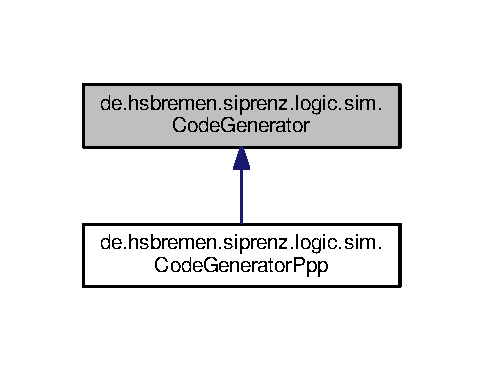
\includegraphics[width=232pt]{interfacede_1_1hsbremen_1_1siprenz_1_1logic_1_1sim_1_1CodeGenerator__inherit__graph}
\end{center}
\end{figure}
\subsection*{Public Member Functions}
\begin{DoxyCompactItemize}
\item 
void \hyperlink{interfacede_1_1hsbremen_1_1siprenz_1_1logic_1_1sim_1_1CodeGenerator_a2c30cae9f4f91ca44fa8c7f27aabbdc0}{generate} (\hyperlink{classde_1_1hsbremen_1_1siprenz_1_1model_1_1xml_1_1Simulation}{Simulation} simulation, String dir\+Name)
\end{DoxyCompactItemize}


\subsection{Detailed Description}
The interfaces for code generators. 

\begin{DoxyAuthor}{Author}
David Mittelstädt 
\end{DoxyAuthor}


\subsection{Member Function Documentation}
\index{de\+::hsbremen\+::siprenz\+::logic\+::sim\+::\+Code\+Generator@{de\+::hsbremen\+::siprenz\+::logic\+::sim\+::\+Code\+Generator}!generate@{generate}}
\index{generate@{generate}!de\+::hsbremen\+::siprenz\+::logic\+::sim\+::\+Code\+Generator@{de\+::hsbremen\+::siprenz\+::logic\+::sim\+::\+Code\+Generator}}
\subsubsection[{\texorpdfstring{generate(\+Simulation simulation, String dir\+Name)}{generate(Simulation simulation, String dirName)}}]{\setlength{\rightskip}{0pt plus 5cm}void de.\+hsbremen.\+siprenz.\+logic.\+sim.\+Code\+Generator.\+generate (
\begin{DoxyParamCaption}
\item[{{\bf Simulation}}]{simulation, }
\item[{String}]{dir\+Name}
\end{DoxyParamCaption}
)}\hypertarget{interfacede_1_1hsbremen_1_1siprenz_1_1logic_1_1sim_1_1CodeGenerator_a2c30cae9f4f91ca44fa8c7f27aabbdc0}{}\label{interfacede_1_1hsbremen_1_1siprenz_1_1logic_1_1sim_1_1CodeGenerator_a2c30cae9f4f91ca44fa8c7f27aabbdc0}

\begin{DoxyParams}{Parameters}
{\em simulation} & \\
\hline
{\em dir\+Name} & \\
\hline
\end{DoxyParams}


Implemented in \hyperlink{classde_1_1hsbremen_1_1siprenz_1_1logic_1_1sim_1_1CodeGeneratorPpp_aaa9d8ca4dbc531bab6c2bf25cdfbc792}{de.\+hsbremen.\+siprenz.\+logic.\+sim.\+Code\+Generator\+Ppp}.



The documentation for this interface was generated from the following file\+:\begin{DoxyCompactItemize}
\item 
src/de/hsbremen/siprenz/logic/sim/Code\+Generator.\+java\end{DoxyCompactItemize}

\hypertarget{classde_1_1hsbremen_1_1siprenz_1_1logic_1_1sim_1_1CodeGeneratorPpp}{}\section{de.\+hsbremen.\+siprenz.\+logic.\+sim.\+Code\+Generator\+Ppp Class Reference}
\label{classde_1_1hsbremen_1_1siprenz_1_1logic_1_1sim_1_1CodeGeneratorPpp}\index{de.\+hsbremen.\+siprenz.\+logic.\+sim.\+Code\+Generator\+Ppp@{de.\+hsbremen.\+siprenz.\+logic.\+sim.\+Code\+Generator\+Ppp}}


Implementation of the Code\+Generataor interface for P2P models.  




Inheritance diagram for de.\+hsbremen.\+siprenz.\+logic.\+sim.\+Code\+Generator\+Ppp\+:\nopagebreak
\begin{figure}[H]
\begin{center}
\leavevmode
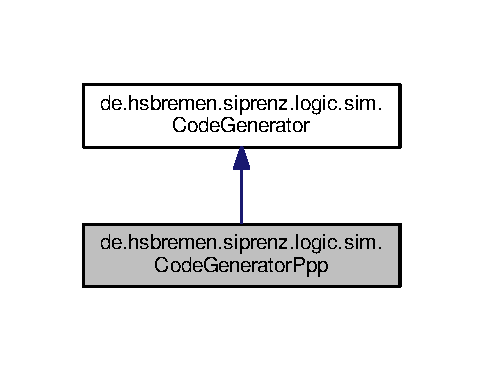
\includegraphics[width=232pt]{classde_1_1hsbremen_1_1siprenz_1_1logic_1_1sim_1_1CodeGeneratorPpp__inherit__graph}
\end{center}
\end{figure}


Collaboration diagram for de.\+hsbremen.\+siprenz.\+logic.\+sim.\+Code\+Generator\+Ppp\+:\nopagebreak
\begin{figure}[H]
\begin{center}
\leavevmode
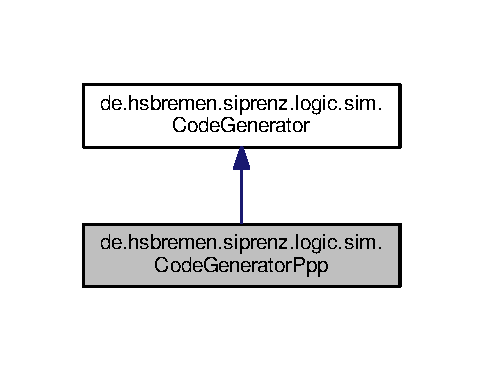
\includegraphics[width=232pt]{classde_1_1hsbremen_1_1siprenz_1_1logic_1_1sim_1_1CodeGeneratorPpp__coll__graph}
\end{center}
\end{figure}
\subsection*{Public Member Functions}
\begin{DoxyCompactItemize}
\item 
void \hyperlink{classde_1_1hsbremen_1_1siprenz_1_1logic_1_1sim_1_1CodeGeneratorPpp_aaa9d8ca4dbc531bab6c2bf25cdfbc792}{generate} (\hyperlink{classde_1_1hsbremen_1_1siprenz_1_1model_1_1xml_1_1Simulation}{Simulation} simulation, String dir\+Name)
\end{DoxyCompactItemize}


\subsection{Detailed Description}
Implementation of the Code\+Generataor interface for P2P models. 

\begin{DoxyAuthor}{Author}
David Mittelstädt 
\end{DoxyAuthor}


\subsection{Member Function Documentation}
\index{de\+::hsbremen\+::siprenz\+::logic\+::sim\+::\+Code\+Generator\+Ppp@{de\+::hsbremen\+::siprenz\+::logic\+::sim\+::\+Code\+Generator\+Ppp}!generate@{generate}}
\index{generate@{generate}!de\+::hsbremen\+::siprenz\+::logic\+::sim\+::\+Code\+Generator\+Ppp@{de\+::hsbremen\+::siprenz\+::logic\+::sim\+::\+Code\+Generator\+Ppp}}
\subsubsection[{\texorpdfstring{generate(\+Simulation simulation, String dir\+Name)}{generate(Simulation simulation, String dirName)}}]{\setlength{\rightskip}{0pt plus 5cm}void de.\+hsbremen.\+siprenz.\+logic.\+sim.\+Code\+Generator\+Ppp.\+generate (
\begin{DoxyParamCaption}
\item[{{\bf Simulation}}]{simulation, }
\item[{String}]{dir\+Name}
\end{DoxyParamCaption}
)\hspace{0.3cm}{\ttfamily [inline]}}\hypertarget{classde_1_1hsbremen_1_1siprenz_1_1logic_1_1sim_1_1CodeGeneratorPpp_aaa9d8ca4dbc531bab6c2bf25cdfbc792}{}\label{classde_1_1hsbremen_1_1siprenz_1_1logic_1_1sim_1_1CodeGeneratorPpp_aaa9d8ca4dbc531bab6c2bf25cdfbc792}

\begin{DoxyParams}{Parameters}
{\em simulation} & \\
\hline
{\em dir\+Name} & \\
\hline
\end{DoxyParams}


Implements \hyperlink{interfacede_1_1hsbremen_1_1siprenz_1_1logic_1_1sim_1_1CodeGenerator_a2c30cae9f4f91ca44fa8c7f27aabbdc0}{de.\+hsbremen.\+siprenz.\+logic.\+sim.\+Code\+Generator}.



The documentation for this class was generated from the following file\+:\begin{DoxyCompactItemize}
\item 
src/de/hsbremen/siprenz/logic/sim/Code\+Generator\+Ppp.\+java\end{DoxyCompactItemize}

\hypertarget{classde_1_1hsbremen_1_1siprenz_1_1model_1_1gen_1_1CodeProps}{}\section{de.\+hsbremen.\+siprenz.\+model.\+gen.\+Code\+Props Class Reference}
\label{classde_1_1hsbremen_1_1siprenz_1_1model_1_1gen_1_1CodeProps}\index{de.\+hsbremen.\+siprenz.\+model.\+gen.\+Code\+Props@{de.\+hsbremen.\+siprenz.\+model.\+gen.\+Code\+Props}}


Class representing code properties.  


\subsection*{Public Member Functions}
\begin{DoxyCompactItemize}
\item 
\hyperlink{classde_1_1hsbremen_1_1siprenz_1_1model_1_1gen_1_1CodeProps_aa966a1d1a7572209a165ecc5de3c59e9}{Code\+Props} (String input\+File, String output\+File)
\begin{DoxyCompactList}\small\item\em Constructor. \end{DoxyCompactList}\item 
String \hyperlink{classde_1_1hsbremen_1_1siprenz_1_1model_1_1gen_1_1CodeProps_a3e1ec80957d2d8737681ddf4f7e54b73}{get\+Input\+File} ()
\begin{DoxyCompactList}\small\item\em Getter-\/method for input\+File. \end{DoxyCompactList}\item 
void \hyperlink{classde_1_1hsbremen_1_1siprenz_1_1model_1_1gen_1_1CodeProps_a2684b89f518f036e177a8a2569f2974f}{set\+Input\+File} (String input\+File)
\begin{DoxyCompactList}\small\item\em Setter-\/method for input\+File. \end{DoxyCompactList}\item 
String \hyperlink{classde_1_1hsbremen_1_1siprenz_1_1model_1_1gen_1_1CodeProps_afe1ad57f346be19f273642dad6ecea3b}{get\+Output\+File} ()
\begin{DoxyCompactList}\small\item\em Getter-\/method for output\+File. \end{DoxyCompactList}\item 
void \hyperlink{classde_1_1hsbremen_1_1siprenz_1_1model_1_1gen_1_1CodeProps_a067699d7b7af723e5e31a99bcc4484cb}{set\+Output\+File} (String output\+File)
\begin{DoxyCompactList}\small\item\em Setter-\/method for output\+File. \end{DoxyCompactList}\end{DoxyCompactItemize}


\subsection{Detailed Description}
Class representing code properties. 

\begin{DoxyAuthor}{Author}
David Mittelstädt 
\end{DoxyAuthor}


\subsection{Constructor \& Destructor Documentation}
\index{de\+::hsbremen\+::siprenz\+::model\+::gen\+::\+Code\+Props@{de\+::hsbremen\+::siprenz\+::model\+::gen\+::\+Code\+Props}!Code\+Props@{Code\+Props}}
\index{Code\+Props@{Code\+Props}!de\+::hsbremen\+::siprenz\+::model\+::gen\+::\+Code\+Props@{de\+::hsbremen\+::siprenz\+::model\+::gen\+::\+Code\+Props}}
\subsubsection[{\texorpdfstring{Code\+Props(\+String input\+File, String output\+File)}{CodeProps(String inputFile, String outputFile)}}]{\setlength{\rightskip}{0pt plus 5cm}de.\+hsbremen.\+siprenz.\+model.\+gen.\+Code\+Props.\+Code\+Props (
\begin{DoxyParamCaption}
\item[{String}]{input\+File, }
\item[{String}]{output\+File}
\end{DoxyParamCaption}
)\hspace{0.3cm}{\ttfamily [inline]}}\hypertarget{classde_1_1hsbremen_1_1siprenz_1_1model_1_1gen_1_1CodeProps_aa966a1d1a7572209a165ecc5de3c59e9}{}\label{classde_1_1hsbremen_1_1siprenz_1_1model_1_1gen_1_1CodeProps_aa966a1d1a7572209a165ecc5de3c59e9}


Constructor. 


\begin{DoxyParams}{Parameters}
{\em input\+File} & Name of the input file \\
\hline
{\em output\+File} & Name of the output file \\
\hline
\end{DoxyParams}


\subsection{Member Function Documentation}
\index{de\+::hsbremen\+::siprenz\+::model\+::gen\+::\+Code\+Props@{de\+::hsbremen\+::siprenz\+::model\+::gen\+::\+Code\+Props}!get\+Input\+File@{get\+Input\+File}}
\index{get\+Input\+File@{get\+Input\+File}!de\+::hsbremen\+::siprenz\+::model\+::gen\+::\+Code\+Props@{de\+::hsbremen\+::siprenz\+::model\+::gen\+::\+Code\+Props}}
\subsubsection[{\texorpdfstring{get\+Input\+File()}{getInputFile()}}]{\setlength{\rightskip}{0pt plus 5cm}String de.\+hsbremen.\+siprenz.\+model.\+gen.\+Code\+Props.\+get\+Input\+File (
\begin{DoxyParamCaption}
{}
\end{DoxyParamCaption}
)\hspace{0.3cm}{\ttfamily [inline]}}\hypertarget{classde_1_1hsbremen_1_1siprenz_1_1model_1_1gen_1_1CodeProps_a3e1ec80957d2d8737681ddf4f7e54b73}{}\label{classde_1_1hsbremen_1_1siprenz_1_1model_1_1gen_1_1CodeProps_a3e1ec80957d2d8737681ddf4f7e54b73}


Getter-\/method for input\+File. 

\begin{DoxyReturn}{Returns}
Name of the input file 
\end{DoxyReturn}
\index{de\+::hsbremen\+::siprenz\+::model\+::gen\+::\+Code\+Props@{de\+::hsbremen\+::siprenz\+::model\+::gen\+::\+Code\+Props}!get\+Output\+File@{get\+Output\+File}}
\index{get\+Output\+File@{get\+Output\+File}!de\+::hsbremen\+::siprenz\+::model\+::gen\+::\+Code\+Props@{de\+::hsbremen\+::siprenz\+::model\+::gen\+::\+Code\+Props}}
\subsubsection[{\texorpdfstring{get\+Output\+File()}{getOutputFile()}}]{\setlength{\rightskip}{0pt plus 5cm}String de.\+hsbremen.\+siprenz.\+model.\+gen.\+Code\+Props.\+get\+Output\+File (
\begin{DoxyParamCaption}
{}
\end{DoxyParamCaption}
)\hspace{0.3cm}{\ttfamily [inline]}}\hypertarget{classde_1_1hsbremen_1_1siprenz_1_1model_1_1gen_1_1CodeProps_afe1ad57f346be19f273642dad6ecea3b}{}\label{classde_1_1hsbremen_1_1siprenz_1_1model_1_1gen_1_1CodeProps_afe1ad57f346be19f273642dad6ecea3b}


Getter-\/method for output\+File. 

\begin{DoxyReturn}{Returns}
Name of the output file 
\end{DoxyReturn}
\index{de\+::hsbremen\+::siprenz\+::model\+::gen\+::\+Code\+Props@{de\+::hsbremen\+::siprenz\+::model\+::gen\+::\+Code\+Props}!set\+Input\+File@{set\+Input\+File}}
\index{set\+Input\+File@{set\+Input\+File}!de\+::hsbremen\+::siprenz\+::model\+::gen\+::\+Code\+Props@{de\+::hsbremen\+::siprenz\+::model\+::gen\+::\+Code\+Props}}
\subsubsection[{\texorpdfstring{set\+Input\+File(\+String input\+File)}{setInputFile(String inputFile)}}]{\setlength{\rightskip}{0pt plus 5cm}void de.\+hsbremen.\+siprenz.\+model.\+gen.\+Code\+Props.\+set\+Input\+File (
\begin{DoxyParamCaption}
\item[{String}]{input\+File}
\end{DoxyParamCaption}
)\hspace{0.3cm}{\ttfamily [inline]}}\hypertarget{classde_1_1hsbremen_1_1siprenz_1_1model_1_1gen_1_1CodeProps_a2684b89f518f036e177a8a2569f2974f}{}\label{classde_1_1hsbremen_1_1siprenz_1_1model_1_1gen_1_1CodeProps_a2684b89f518f036e177a8a2569f2974f}


Setter-\/method for input\+File. 


\begin{DoxyParams}{Parameters}
{\em input\+File} & Name of the input file \\
\hline
\end{DoxyParams}
\index{de\+::hsbremen\+::siprenz\+::model\+::gen\+::\+Code\+Props@{de\+::hsbremen\+::siprenz\+::model\+::gen\+::\+Code\+Props}!set\+Output\+File@{set\+Output\+File}}
\index{set\+Output\+File@{set\+Output\+File}!de\+::hsbremen\+::siprenz\+::model\+::gen\+::\+Code\+Props@{de\+::hsbremen\+::siprenz\+::model\+::gen\+::\+Code\+Props}}
\subsubsection[{\texorpdfstring{set\+Output\+File(\+String output\+File)}{setOutputFile(String outputFile)}}]{\setlength{\rightskip}{0pt plus 5cm}void de.\+hsbremen.\+siprenz.\+model.\+gen.\+Code\+Props.\+set\+Output\+File (
\begin{DoxyParamCaption}
\item[{String}]{output\+File}
\end{DoxyParamCaption}
)\hspace{0.3cm}{\ttfamily [inline]}}\hypertarget{classde_1_1hsbremen_1_1siprenz_1_1model_1_1gen_1_1CodeProps_a067699d7b7af723e5e31a99bcc4484cb}{}\label{classde_1_1hsbremen_1_1siprenz_1_1model_1_1gen_1_1CodeProps_a067699d7b7af723e5e31a99bcc4484cb}


Setter-\/method for output\+File. 


\begin{DoxyParams}{Parameters}
{\em output\+File} & Name of the output file \\
\hline
\end{DoxyParams}


The documentation for this class was generated from the following file\+:\begin{DoxyCompactItemize}
\item 
src/de/hsbremen/siprenz/model/gen/Code\+Props.\+java\end{DoxyCompactItemize}

\hypertarget{classde_1_1hsbremen_1_1siprenz_1_1model_1_1xml_1_1Connection}{}\section{de.\+hsbremen.\+siprenz.\+model.\+xml.\+Connection Class Reference}
\label{classde_1_1hsbremen_1_1siprenz_1_1model_1_1xml_1_1Connection}\index{de.\+hsbremen.\+siprenz.\+model.\+xml.\+Connection@{de.\+hsbremen.\+siprenz.\+model.\+xml.\+Connection}}


Class for connection element of the simulation.  


\subsection*{Public Member Functions}
\begin{DoxyCompactItemize}
\item 
\hyperlink{classde_1_1hsbremen_1_1siprenz_1_1model_1_1xml_1_1Connection_a2ba40a1c400262437eb0246ae869e9f8}{Connection} ()\hypertarget{classde_1_1hsbremen_1_1siprenz_1_1model_1_1xml_1_1Connection_a2ba40a1c400262437eb0246ae869e9f8}{}\label{classde_1_1hsbremen_1_1siprenz_1_1model_1_1xml_1_1Connection_a2ba40a1c400262437eb0246ae869e9f8}

\begin{DoxyCompactList}\small\item\em Default constructor. \end{DoxyCompactList}\item 
\hyperlink{classde_1_1hsbremen_1_1siprenz_1_1model_1_1xml_1_1Connection_a4ce0b9a5a1d9e20078bff797671eabe5}{Connection} (\hyperlink{classde_1_1hsbremen_1_1siprenz_1_1model_1_1xml_1_1Node}{Node} source, \hyperlink{classde_1_1hsbremen_1_1siprenz_1_1model_1_1xml_1_1Node}{Node} destination, String type, String data\+Rate, String delay, String ip, String subnet)
\begin{DoxyCompactList}\small\item\em Constructor with all attributes. \end{DoxyCompactList}\item 
\hyperlink{classde_1_1hsbremen_1_1siprenz_1_1model_1_1xml_1_1Node}{Node} \hyperlink{classde_1_1hsbremen_1_1siprenz_1_1model_1_1xml_1_1Connection_a406342644ccdbd291fbfe5500a019b4a}{get\+Source} ()
\item 
void \hyperlink{classde_1_1hsbremen_1_1siprenz_1_1model_1_1xml_1_1Connection_a6c7004b65a1f965aff92ebc0dc968d0f}{set\+Source} (\hyperlink{classde_1_1hsbremen_1_1siprenz_1_1model_1_1xml_1_1Node}{Node} source)
\item 
\hyperlink{classde_1_1hsbremen_1_1siprenz_1_1model_1_1xml_1_1Node}{Node} \hyperlink{classde_1_1hsbremen_1_1siprenz_1_1model_1_1xml_1_1Connection_a5373ca2592ef4594fccf0997c0788374}{get\+Destination} ()
\item 
void \hyperlink{classde_1_1hsbremen_1_1siprenz_1_1model_1_1xml_1_1Connection_a21ca377ff86403f392263222f71fce74}{set\+Destination} (\hyperlink{classde_1_1hsbremen_1_1siprenz_1_1model_1_1xml_1_1Node}{Node} destination)
\item 
String \hyperlink{classde_1_1hsbremen_1_1siprenz_1_1model_1_1xml_1_1Connection_aded733298efa107776870518d1e1f62b}{get\+Type} ()
\item 
void \hyperlink{classde_1_1hsbremen_1_1siprenz_1_1model_1_1xml_1_1Connection_afe77af3528d52913b64300ca19a8cc89}{set\+Type} (String type)
\item 
String \hyperlink{classde_1_1hsbremen_1_1siprenz_1_1model_1_1xml_1_1Connection_ae9f65d4e866d7fefc3abb04f6509339c}{get\+Data\+Rate} ()
\item 
void \hyperlink{classde_1_1hsbremen_1_1siprenz_1_1model_1_1xml_1_1Connection_ae03544a676a56ecce7096cc1289ddc98}{set\+Data\+Rate} (String data\+Rate)
\item 
String \hyperlink{classde_1_1hsbremen_1_1siprenz_1_1model_1_1xml_1_1Connection_ab218b1b4de16bbb1b735b850d26ffe79}{get\+Delay} ()
\item 
void \hyperlink{classde_1_1hsbremen_1_1siprenz_1_1model_1_1xml_1_1Connection_ac683705c2b3c99d564a40e7893ff3b52}{set\+Delay} (String delay)
\item 
String \hyperlink{classde_1_1hsbremen_1_1siprenz_1_1model_1_1xml_1_1Connection_a8ef577b35fa507a9a1be48d5f7f0a599}{get\+Ip} ()
\item 
void \hyperlink{classde_1_1hsbremen_1_1siprenz_1_1model_1_1xml_1_1Connection_a148d6f5704ef2c1391e0238fc770c0e7}{set\+Ip} (String ip)
\item 
String \hyperlink{classde_1_1hsbremen_1_1siprenz_1_1model_1_1xml_1_1Connection_a236028678fa730814118e1f947b4abed}{get\+Subnet} ()
\item 
void \hyperlink{classde_1_1hsbremen_1_1siprenz_1_1model_1_1xml_1_1Connection_ad0cd420838d99db231eec532631abf04}{set\+Subnet} (String subnet)
\end{DoxyCompactItemize}


\subsection{Detailed Description}
Class for connection element of the simulation. 

This class represents the connection object of the simulation. Uses annotations for X\+ML support.

\begin{DoxyAuthor}{Author}
David Mittelstädt 
\end{DoxyAuthor}


\subsection{Constructor \& Destructor Documentation}
\index{de\+::hsbremen\+::siprenz\+::model\+::xml\+::\+Connection@{de\+::hsbremen\+::siprenz\+::model\+::xml\+::\+Connection}!Connection@{Connection}}
\index{Connection@{Connection}!de\+::hsbremen\+::siprenz\+::model\+::xml\+::\+Connection@{de\+::hsbremen\+::siprenz\+::model\+::xml\+::\+Connection}}
\subsubsection[{\texorpdfstring{Connection(\+Node source, Node destination, String type, String data\+Rate, String delay, String ip, String subnet)}{Connection(Node source, Node destination, String type, String dataRate, String delay, String ip, String subnet)}}]{\setlength{\rightskip}{0pt plus 5cm}de.\+hsbremen.\+siprenz.\+model.\+xml.\+Connection.\+Connection (
\begin{DoxyParamCaption}
\item[{{\bf Node}}]{source, }
\item[{{\bf Node}}]{destination, }
\item[{String}]{type, }
\item[{String}]{data\+Rate, }
\item[{String}]{delay, }
\item[{String}]{ip, }
\item[{String}]{subnet}
\end{DoxyParamCaption}
)\hspace{0.3cm}{\ttfamily [inline]}}\hypertarget{classde_1_1hsbremen_1_1siprenz_1_1model_1_1xml_1_1Connection_a4ce0b9a5a1d9e20078bff797671eabe5}{}\label{classde_1_1hsbremen_1_1siprenz_1_1model_1_1xml_1_1Connection_a4ce0b9a5a1d9e20078bff797671eabe5}


Constructor with all attributes. 


\begin{DoxyParams}{Parameters}
{\em source} & Source node \\
\hline
{\em destination} & Destination node \\
\hline
{\em type} & connection type, e.\+g. P2P \\
\hline
{\em data\+Rate} & Data rate \\
\hline
{\em delay} & delay of the connection \\
\hline
{\em ip} & first IP of the given nodes \\
\hline
{\em subnet} & subnet mask \\
\hline
\end{DoxyParams}


\subsection{Member Function Documentation}
\index{de\+::hsbremen\+::siprenz\+::model\+::xml\+::\+Connection@{de\+::hsbremen\+::siprenz\+::model\+::xml\+::\+Connection}!get\+Data\+Rate@{get\+Data\+Rate}}
\index{get\+Data\+Rate@{get\+Data\+Rate}!de\+::hsbremen\+::siprenz\+::model\+::xml\+::\+Connection@{de\+::hsbremen\+::siprenz\+::model\+::xml\+::\+Connection}}
\subsubsection[{\texorpdfstring{get\+Data\+Rate()}{getDataRate()}}]{\setlength{\rightskip}{0pt plus 5cm}String de.\+hsbremen.\+siprenz.\+model.\+xml.\+Connection.\+get\+Data\+Rate (
\begin{DoxyParamCaption}
{}
\end{DoxyParamCaption}
)\hspace{0.3cm}{\ttfamily [inline]}}\hypertarget{classde_1_1hsbremen_1_1siprenz_1_1model_1_1xml_1_1Connection_ae9f65d4e866d7fefc3abb04f6509339c}{}\label{classde_1_1hsbremen_1_1siprenz_1_1model_1_1xml_1_1Connection_ae9f65d4e866d7fefc3abb04f6509339c}
\begin{DoxyReturn}{Returns}
Data rate 
\end{DoxyReturn}
\index{de\+::hsbremen\+::siprenz\+::model\+::xml\+::\+Connection@{de\+::hsbremen\+::siprenz\+::model\+::xml\+::\+Connection}!get\+Delay@{get\+Delay}}
\index{get\+Delay@{get\+Delay}!de\+::hsbremen\+::siprenz\+::model\+::xml\+::\+Connection@{de\+::hsbremen\+::siprenz\+::model\+::xml\+::\+Connection}}
\subsubsection[{\texorpdfstring{get\+Delay()}{getDelay()}}]{\setlength{\rightskip}{0pt plus 5cm}String de.\+hsbremen.\+siprenz.\+model.\+xml.\+Connection.\+get\+Delay (
\begin{DoxyParamCaption}
{}
\end{DoxyParamCaption}
)\hspace{0.3cm}{\ttfamily [inline]}}\hypertarget{classde_1_1hsbremen_1_1siprenz_1_1model_1_1xml_1_1Connection_ab218b1b4de16bbb1b735b850d26ffe79}{}\label{classde_1_1hsbremen_1_1siprenz_1_1model_1_1xml_1_1Connection_ab218b1b4de16bbb1b735b850d26ffe79}
\begin{DoxyReturn}{Returns}
delay of the connection 
\end{DoxyReturn}
\index{de\+::hsbremen\+::siprenz\+::model\+::xml\+::\+Connection@{de\+::hsbremen\+::siprenz\+::model\+::xml\+::\+Connection}!get\+Destination@{get\+Destination}}
\index{get\+Destination@{get\+Destination}!de\+::hsbremen\+::siprenz\+::model\+::xml\+::\+Connection@{de\+::hsbremen\+::siprenz\+::model\+::xml\+::\+Connection}}
\subsubsection[{\texorpdfstring{get\+Destination()}{getDestination()}}]{\setlength{\rightskip}{0pt plus 5cm}{\bf Node} de.\+hsbremen.\+siprenz.\+model.\+xml.\+Connection.\+get\+Destination (
\begin{DoxyParamCaption}
{}
\end{DoxyParamCaption}
)\hspace{0.3cm}{\ttfamily [inline]}}\hypertarget{classde_1_1hsbremen_1_1siprenz_1_1model_1_1xml_1_1Connection_a5373ca2592ef4594fccf0997c0788374}{}\label{classde_1_1hsbremen_1_1siprenz_1_1model_1_1xml_1_1Connection_a5373ca2592ef4594fccf0997c0788374}
\begin{DoxyReturn}{Returns}
Destination node 
\end{DoxyReturn}
\index{de\+::hsbremen\+::siprenz\+::model\+::xml\+::\+Connection@{de\+::hsbremen\+::siprenz\+::model\+::xml\+::\+Connection}!get\+Ip@{get\+Ip}}
\index{get\+Ip@{get\+Ip}!de\+::hsbremen\+::siprenz\+::model\+::xml\+::\+Connection@{de\+::hsbremen\+::siprenz\+::model\+::xml\+::\+Connection}}
\subsubsection[{\texorpdfstring{get\+Ip()}{getIp()}}]{\setlength{\rightskip}{0pt plus 5cm}String de.\+hsbremen.\+siprenz.\+model.\+xml.\+Connection.\+get\+Ip (
\begin{DoxyParamCaption}
{}
\end{DoxyParamCaption}
)\hspace{0.3cm}{\ttfamily [inline]}}\hypertarget{classde_1_1hsbremen_1_1siprenz_1_1model_1_1xml_1_1Connection_a8ef577b35fa507a9a1be48d5f7f0a599}{}\label{classde_1_1hsbremen_1_1siprenz_1_1model_1_1xml_1_1Connection_a8ef577b35fa507a9a1be48d5f7f0a599}
\begin{DoxyReturn}{Returns}
first IP of the given nodes 
\end{DoxyReturn}
\index{de\+::hsbremen\+::siprenz\+::model\+::xml\+::\+Connection@{de\+::hsbremen\+::siprenz\+::model\+::xml\+::\+Connection}!get\+Source@{get\+Source}}
\index{get\+Source@{get\+Source}!de\+::hsbremen\+::siprenz\+::model\+::xml\+::\+Connection@{de\+::hsbremen\+::siprenz\+::model\+::xml\+::\+Connection}}
\subsubsection[{\texorpdfstring{get\+Source()}{getSource()}}]{\setlength{\rightskip}{0pt plus 5cm}{\bf Node} de.\+hsbremen.\+siprenz.\+model.\+xml.\+Connection.\+get\+Source (
\begin{DoxyParamCaption}
{}
\end{DoxyParamCaption}
)\hspace{0.3cm}{\ttfamily [inline]}}\hypertarget{classde_1_1hsbremen_1_1siprenz_1_1model_1_1xml_1_1Connection_a406342644ccdbd291fbfe5500a019b4a}{}\label{classde_1_1hsbremen_1_1siprenz_1_1model_1_1xml_1_1Connection_a406342644ccdbd291fbfe5500a019b4a}
\begin{DoxyReturn}{Returns}
Source node 
\end{DoxyReturn}
\index{de\+::hsbremen\+::siprenz\+::model\+::xml\+::\+Connection@{de\+::hsbremen\+::siprenz\+::model\+::xml\+::\+Connection}!get\+Subnet@{get\+Subnet}}
\index{get\+Subnet@{get\+Subnet}!de\+::hsbremen\+::siprenz\+::model\+::xml\+::\+Connection@{de\+::hsbremen\+::siprenz\+::model\+::xml\+::\+Connection}}
\subsubsection[{\texorpdfstring{get\+Subnet()}{getSubnet()}}]{\setlength{\rightskip}{0pt plus 5cm}String de.\+hsbremen.\+siprenz.\+model.\+xml.\+Connection.\+get\+Subnet (
\begin{DoxyParamCaption}
{}
\end{DoxyParamCaption}
)\hspace{0.3cm}{\ttfamily [inline]}}\hypertarget{classde_1_1hsbremen_1_1siprenz_1_1model_1_1xml_1_1Connection_a236028678fa730814118e1f947b4abed}{}\label{classde_1_1hsbremen_1_1siprenz_1_1model_1_1xml_1_1Connection_a236028678fa730814118e1f947b4abed}
\begin{DoxyReturn}{Returns}
subnet mask 
\end{DoxyReturn}
\index{de\+::hsbremen\+::siprenz\+::model\+::xml\+::\+Connection@{de\+::hsbremen\+::siprenz\+::model\+::xml\+::\+Connection}!get\+Type@{get\+Type}}
\index{get\+Type@{get\+Type}!de\+::hsbremen\+::siprenz\+::model\+::xml\+::\+Connection@{de\+::hsbremen\+::siprenz\+::model\+::xml\+::\+Connection}}
\subsubsection[{\texorpdfstring{get\+Type()}{getType()}}]{\setlength{\rightskip}{0pt plus 5cm}String de.\+hsbremen.\+siprenz.\+model.\+xml.\+Connection.\+get\+Type (
\begin{DoxyParamCaption}
{}
\end{DoxyParamCaption}
)\hspace{0.3cm}{\ttfamily [inline]}}\hypertarget{classde_1_1hsbremen_1_1siprenz_1_1model_1_1xml_1_1Connection_aded733298efa107776870518d1e1f62b}{}\label{classde_1_1hsbremen_1_1siprenz_1_1model_1_1xml_1_1Connection_aded733298efa107776870518d1e1f62b}
\begin{DoxyReturn}{Returns}
connection type 
\end{DoxyReturn}
\index{de\+::hsbremen\+::siprenz\+::model\+::xml\+::\+Connection@{de\+::hsbremen\+::siprenz\+::model\+::xml\+::\+Connection}!set\+Data\+Rate@{set\+Data\+Rate}}
\index{set\+Data\+Rate@{set\+Data\+Rate}!de\+::hsbremen\+::siprenz\+::model\+::xml\+::\+Connection@{de\+::hsbremen\+::siprenz\+::model\+::xml\+::\+Connection}}
\subsubsection[{\texorpdfstring{set\+Data\+Rate(\+String data\+Rate)}{setDataRate(String dataRate)}}]{\setlength{\rightskip}{0pt plus 5cm}void de.\+hsbremen.\+siprenz.\+model.\+xml.\+Connection.\+set\+Data\+Rate (
\begin{DoxyParamCaption}
\item[{String}]{data\+Rate}
\end{DoxyParamCaption}
)\hspace{0.3cm}{\ttfamily [inline]}}\hypertarget{classde_1_1hsbremen_1_1siprenz_1_1model_1_1xml_1_1Connection_ae03544a676a56ecce7096cc1289ddc98}{}\label{classde_1_1hsbremen_1_1siprenz_1_1model_1_1xml_1_1Connection_ae03544a676a56ecce7096cc1289ddc98}

\begin{DoxyParams}{Parameters}
{\em data\+Rate} & Data rate \\
\hline
\end{DoxyParams}
\index{de\+::hsbremen\+::siprenz\+::model\+::xml\+::\+Connection@{de\+::hsbremen\+::siprenz\+::model\+::xml\+::\+Connection}!set\+Delay@{set\+Delay}}
\index{set\+Delay@{set\+Delay}!de\+::hsbremen\+::siprenz\+::model\+::xml\+::\+Connection@{de\+::hsbremen\+::siprenz\+::model\+::xml\+::\+Connection}}
\subsubsection[{\texorpdfstring{set\+Delay(\+String delay)}{setDelay(String delay)}}]{\setlength{\rightskip}{0pt plus 5cm}void de.\+hsbremen.\+siprenz.\+model.\+xml.\+Connection.\+set\+Delay (
\begin{DoxyParamCaption}
\item[{String}]{delay}
\end{DoxyParamCaption}
)\hspace{0.3cm}{\ttfamily [inline]}}\hypertarget{classde_1_1hsbremen_1_1siprenz_1_1model_1_1xml_1_1Connection_ac683705c2b3c99d564a40e7893ff3b52}{}\label{classde_1_1hsbremen_1_1siprenz_1_1model_1_1xml_1_1Connection_ac683705c2b3c99d564a40e7893ff3b52}

\begin{DoxyParams}{Parameters}
{\em delay} & delay of the connection \\
\hline
\end{DoxyParams}
\index{de\+::hsbremen\+::siprenz\+::model\+::xml\+::\+Connection@{de\+::hsbremen\+::siprenz\+::model\+::xml\+::\+Connection}!set\+Destination@{set\+Destination}}
\index{set\+Destination@{set\+Destination}!de\+::hsbremen\+::siprenz\+::model\+::xml\+::\+Connection@{de\+::hsbremen\+::siprenz\+::model\+::xml\+::\+Connection}}
\subsubsection[{\texorpdfstring{set\+Destination(\+Node destination)}{setDestination(Node destination)}}]{\setlength{\rightskip}{0pt plus 5cm}void de.\+hsbremen.\+siprenz.\+model.\+xml.\+Connection.\+set\+Destination (
\begin{DoxyParamCaption}
\item[{{\bf Node}}]{destination}
\end{DoxyParamCaption}
)\hspace{0.3cm}{\ttfamily [inline]}}\hypertarget{classde_1_1hsbremen_1_1siprenz_1_1model_1_1xml_1_1Connection_a21ca377ff86403f392263222f71fce74}{}\label{classde_1_1hsbremen_1_1siprenz_1_1model_1_1xml_1_1Connection_a21ca377ff86403f392263222f71fce74}

\begin{DoxyParams}{Parameters}
{\em destination} & Destination node \\
\hline
\end{DoxyParams}
\index{de\+::hsbremen\+::siprenz\+::model\+::xml\+::\+Connection@{de\+::hsbremen\+::siprenz\+::model\+::xml\+::\+Connection}!set\+Ip@{set\+Ip}}
\index{set\+Ip@{set\+Ip}!de\+::hsbremen\+::siprenz\+::model\+::xml\+::\+Connection@{de\+::hsbremen\+::siprenz\+::model\+::xml\+::\+Connection}}
\subsubsection[{\texorpdfstring{set\+Ip(\+String ip)}{setIp(String ip)}}]{\setlength{\rightskip}{0pt plus 5cm}void de.\+hsbremen.\+siprenz.\+model.\+xml.\+Connection.\+set\+Ip (
\begin{DoxyParamCaption}
\item[{String}]{ip}
\end{DoxyParamCaption}
)\hspace{0.3cm}{\ttfamily [inline]}}\hypertarget{classde_1_1hsbremen_1_1siprenz_1_1model_1_1xml_1_1Connection_a148d6f5704ef2c1391e0238fc770c0e7}{}\label{classde_1_1hsbremen_1_1siprenz_1_1model_1_1xml_1_1Connection_a148d6f5704ef2c1391e0238fc770c0e7}

\begin{DoxyParams}{Parameters}
{\em ip} & first IP of the given nodes \\
\hline
\end{DoxyParams}
\index{de\+::hsbremen\+::siprenz\+::model\+::xml\+::\+Connection@{de\+::hsbremen\+::siprenz\+::model\+::xml\+::\+Connection}!set\+Source@{set\+Source}}
\index{set\+Source@{set\+Source}!de\+::hsbremen\+::siprenz\+::model\+::xml\+::\+Connection@{de\+::hsbremen\+::siprenz\+::model\+::xml\+::\+Connection}}
\subsubsection[{\texorpdfstring{set\+Source(\+Node source)}{setSource(Node source)}}]{\setlength{\rightskip}{0pt plus 5cm}void de.\+hsbremen.\+siprenz.\+model.\+xml.\+Connection.\+set\+Source (
\begin{DoxyParamCaption}
\item[{{\bf Node}}]{source}
\end{DoxyParamCaption}
)\hspace{0.3cm}{\ttfamily [inline]}}\hypertarget{classde_1_1hsbremen_1_1siprenz_1_1model_1_1xml_1_1Connection_a6c7004b65a1f965aff92ebc0dc968d0f}{}\label{classde_1_1hsbremen_1_1siprenz_1_1model_1_1xml_1_1Connection_a6c7004b65a1f965aff92ebc0dc968d0f}

\begin{DoxyParams}{Parameters}
{\em source} & Source node \\
\hline
\end{DoxyParams}
\index{de\+::hsbremen\+::siprenz\+::model\+::xml\+::\+Connection@{de\+::hsbremen\+::siprenz\+::model\+::xml\+::\+Connection}!set\+Subnet@{set\+Subnet}}
\index{set\+Subnet@{set\+Subnet}!de\+::hsbremen\+::siprenz\+::model\+::xml\+::\+Connection@{de\+::hsbremen\+::siprenz\+::model\+::xml\+::\+Connection}}
\subsubsection[{\texorpdfstring{set\+Subnet(\+String subnet)}{setSubnet(String subnet)}}]{\setlength{\rightskip}{0pt plus 5cm}void de.\+hsbremen.\+siprenz.\+model.\+xml.\+Connection.\+set\+Subnet (
\begin{DoxyParamCaption}
\item[{String}]{subnet}
\end{DoxyParamCaption}
)\hspace{0.3cm}{\ttfamily [inline]}}\hypertarget{classde_1_1hsbremen_1_1siprenz_1_1model_1_1xml_1_1Connection_ad0cd420838d99db231eec532631abf04}{}\label{classde_1_1hsbremen_1_1siprenz_1_1model_1_1xml_1_1Connection_ad0cd420838d99db231eec532631abf04}

\begin{DoxyParams}{Parameters}
{\em subnet} & subnet mask \\
\hline
\end{DoxyParams}
\index{de\+::hsbremen\+::siprenz\+::model\+::xml\+::\+Connection@{de\+::hsbremen\+::siprenz\+::model\+::xml\+::\+Connection}!set\+Type@{set\+Type}}
\index{set\+Type@{set\+Type}!de\+::hsbremen\+::siprenz\+::model\+::xml\+::\+Connection@{de\+::hsbremen\+::siprenz\+::model\+::xml\+::\+Connection}}
\subsubsection[{\texorpdfstring{set\+Type(\+String type)}{setType(String type)}}]{\setlength{\rightskip}{0pt plus 5cm}void de.\+hsbremen.\+siprenz.\+model.\+xml.\+Connection.\+set\+Type (
\begin{DoxyParamCaption}
\item[{String}]{type}
\end{DoxyParamCaption}
)\hspace{0.3cm}{\ttfamily [inline]}}\hypertarget{classde_1_1hsbremen_1_1siprenz_1_1model_1_1xml_1_1Connection_afe77af3528d52913b64300ca19a8cc89}{}\label{classde_1_1hsbremen_1_1siprenz_1_1model_1_1xml_1_1Connection_afe77af3528d52913b64300ca19a8cc89}

\begin{DoxyParams}{Parameters}
{\em type} & connection type \\
\hline
\end{DoxyParams}


The documentation for this class was generated from the following file\+:\begin{DoxyCompactItemize}
\item 
src/de/hsbremen/siprenz/model/xml/Connection.\+java\end{DoxyCompactItemize}

\hypertarget{classde_1_1hsbremen_1_1siprenz_1_1controller_1_1Controller}{}\section{de.\+hsbremen.\+siprenz.\+controller.\+Controller Class Reference}
\label{classde_1_1hsbremen_1_1siprenz_1_1controller_1_1Controller}\index{de.\+hsbremen.\+siprenz.\+controller.\+Controller@{de.\+hsbremen.\+siprenz.\+controller.\+Controller}}


The controller of the Sim\+Gen-\/\+Tool.  


\subsection*{Public Member Functions}
\begin{DoxyCompactItemize}
\item 
\hyperlink{classde_1_1hsbremen_1_1siprenz_1_1controller_1_1Controller_a79d6ea7bfe78c9ffff28c4e52eadab75}{Controller} (String args\mbox{[}$\,$\mbox{]})
\begin{DoxyCompactList}\small\item\em Constructor. \end{DoxyCompactList}\item 
void {\bfseries copy} ()\hypertarget{classde_1_1hsbremen_1_1siprenz_1_1controller_1_1Controller_a0f28a729a0d15adebaf8ca6e52e181cb}{}\label{classde_1_1hsbremen_1_1siprenz_1_1controller_1_1Controller_a0f28a729a0d15adebaf8ca6e52e181cb}

\item 
void \hyperlink{classde_1_1hsbremen_1_1siprenz_1_1controller_1_1Controller_aaa3798b73eec3e58ce26f944a9deaba5}{start} ()
\begin{DoxyCompactList}\small\item\em Function to start the controller. \end{DoxyCompactList}\end{DoxyCompactItemize}


\subsection{Detailed Description}
The controller of the Sim\+Gen-\/\+Tool. 

This class controls the flow of the program and calls the different functions of the other classes.

\begin{DoxyAuthor}{Author}
David Mittelstädt 
\end{DoxyAuthor}


\subsection{Constructor \& Destructor Documentation}
\index{de\+::hsbremen\+::siprenz\+::controller\+::\+Controller@{de\+::hsbremen\+::siprenz\+::controller\+::\+Controller}!Controller@{Controller}}
\index{Controller@{Controller}!de\+::hsbremen\+::siprenz\+::controller\+::\+Controller@{de\+::hsbremen\+::siprenz\+::controller\+::\+Controller}}
\subsubsection[{\texorpdfstring{Controller(\+String args[])}{Controller(String args[])}}]{\setlength{\rightskip}{0pt plus 5cm}de.\+hsbremen.\+siprenz.\+controller.\+Controller.\+Controller (
\begin{DoxyParamCaption}
\item[{String}]{args\mbox{[}$\,$\mbox{]}}
\end{DoxyParamCaption}
)\hspace{0.3cm}{\ttfamily [inline]}}\hypertarget{classde_1_1hsbremen_1_1siprenz_1_1controller_1_1Controller_a79d6ea7bfe78c9ffff28c4e52eadab75}{}\label{classde_1_1hsbremen_1_1siprenz_1_1controller_1_1Controller_a79d6ea7bfe78c9ffff28c4e52eadab75}


Constructor. 

Calls the initialization of this class


\begin{DoxyParams}{Parameters}
{\em args} & arguments given from the command-\/line \\
\hline
\end{DoxyParams}


\subsection{Member Function Documentation}
\index{de\+::hsbremen\+::siprenz\+::controller\+::\+Controller@{de\+::hsbremen\+::siprenz\+::controller\+::\+Controller}!start@{start}}
\index{start@{start}!de\+::hsbremen\+::siprenz\+::controller\+::\+Controller@{de\+::hsbremen\+::siprenz\+::controller\+::\+Controller}}
\subsubsection[{\texorpdfstring{start()}{start()}}]{\setlength{\rightskip}{0pt plus 5cm}void de.\+hsbremen.\+siprenz.\+controller.\+Controller.\+start (
\begin{DoxyParamCaption}
{}
\end{DoxyParamCaption}
)\hspace{0.3cm}{\ttfamily [inline]}}\hypertarget{classde_1_1hsbremen_1_1siprenz_1_1controller_1_1Controller_aaa3798b73eec3e58ce26f944a9deaba5}{}\label{classde_1_1hsbremen_1_1siprenz_1_1controller_1_1Controller_aaa3798b73eec3e58ce26f944a9deaba5}


Function to start the controller. 

Only functions which can be called from other classes 

The documentation for this class was generated from the following file\+:\begin{DoxyCompactItemize}
\item 
src/de/hsbremen/siprenz/controller/Controller.\+java\end{DoxyCompactItemize}

\hypertarget{classde_1_1hsbremen_1_1siprenz_1_1utils_1_1FileUtils}{}\section{de.\+hsbremen.\+siprenz.\+utils.\+File\+Utils Class Reference}
\label{classde_1_1hsbremen_1_1siprenz_1_1utils_1_1FileUtils}\index{de.\+hsbremen.\+siprenz.\+utils.\+File\+Utils@{de.\+hsbremen.\+siprenz.\+utils.\+File\+Utils}}


Class for file and directory operations.  


\subsection*{Static Public Member Functions}
\begin{DoxyCompactItemize}
\item 
static boolean \hyperlink{classde_1_1hsbremen_1_1siprenz_1_1utils_1_1FileUtils_a9b43144fe6eeb361624d509d4bf500ce}{is\+File} (String file\+Name)
\item 
static void \hyperlink{classde_1_1hsbremen_1_1siprenz_1_1utils_1_1FileUtils_a101a622a781056e119c9ee1de1c4cf94}{create\+File} (String to\+Write, String path\+Name)
\begin{DoxyCompactList}\small\item\em Creating a new File with given content. \end{DoxyCompactList}\item 
static boolean \hyperlink{classde_1_1hsbremen_1_1siprenz_1_1utils_1_1FileUtils_aca7379519688339682d22353d724cb88}{create\+Dir} (String dir\+Name)
\begin{DoxyCompactList}\small\item\em Creating a directory. \end{DoxyCompactList}\item 
static boolean \hyperlink{classde_1_1hsbremen_1_1siprenz_1_1utils_1_1FileUtils_a5aec54ce389ce7d4e2dadad1aff0b0bc}{create\+Dirs} (String dir\+Path)
\begin{DoxyCompactList}\small\item\em Creating a directory tree if parent directory doesn\textquotesingle{}t exist. \end{DoxyCompactList}\item 
static boolean \hyperlink{classde_1_1hsbremen_1_1siprenz_1_1utils_1_1FileUtils_a22c3f496d3e6878705542d37bd419b81}{is\+Dir} (String dir\+Name)
\begin{DoxyCompactList}\small\item\em Checks existing directory. \end{DoxyCompactList}\item 
static void \hyperlink{classde_1_1hsbremen_1_1siprenz_1_1utils_1_1FileUtils_a6ab1fc80abb5196aa246d9026a75ed7a}{delete\+Dir} (String dir\+Name)  throws I\+O\+Exception 
\begin{DoxyCompactList}\small\item\em Deleting recursively directories. \end{DoxyCompactList}\end{DoxyCompactItemize}


\subsection{Detailed Description}
Class for file and directory operations. 

\begin{DoxyAuthor}{Author}
David Mittelstädt 
\end{DoxyAuthor}


\subsection{Member Function Documentation}
\index{de\+::hsbremen\+::siprenz\+::utils\+::\+File\+Utils@{de\+::hsbremen\+::siprenz\+::utils\+::\+File\+Utils}!create\+Dir@{create\+Dir}}
\index{create\+Dir@{create\+Dir}!de\+::hsbremen\+::siprenz\+::utils\+::\+File\+Utils@{de\+::hsbremen\+::siprenz\+::utils\+::\+File\+Utils}}
\subsubsection[{\texorpdfstring{create\+Dir(\+String dir\+Name)}{createDir(String dirName)}}]{\setlength{\rightskip}{0pt plus 5cm}static boolean de.\+hsbremen.\+siprenz.\+utils.\+File\+Utils.\+create\+Dir (
\begin{DoxyParamCaption}
\item[{String}]{dir\+Name}
\end{DoxyParamCaption}
)\hspace{0.3cm}{\ttfamily [inline]}, {\ttfamily [static]}}\hypertarget{classde_1_1hsbremen_1_1siprenz_1_1utils_1_1FileUtils_aca7379519688339682d22353d724cb88}{}\label{classde_1_1hsbremen_1_1siprenz_1_1utils_1_1FileUtils_aca7379519688339682d22353d724cb88}


Creating a directory. 


\begin{DoxyParams}{Parameters}
{\em dir\+Name} & name of the directory \\
\hline
\end{DoxyParams}
\begin{DoxyReturn}{Returns}
whether directory was successfully created 
\end{DoxyReturn}
\index{de\+::hsbremen\+::siprenz\+::utils\+::\+File\+Utils@{de\+::hsbremen\+::siprenz\+::utils\+::\+File\+Utils}!create\+Dirs@{create\+Dirs}}
\index{create\+Dirs@{create\+Dirs}!de\+::hsbremen\+::siprenz\+::utils\+::\+File\+Utils@{de\+::hsbremen\+::siprenz\+::utils\+::\+File\+Utils}}
\subsubsection[{\texorpdfstring{create\+Dirs(\+String dir\+Path)}{createDirs(String dirPath)}}]{\setlength{\rightskip}{0pt plus 5cm}static boolean de.\+hsbremen.\+siprenz.\+utils.\+File\+Utils.\+create\+Dirs (
\begin{DoxyParamCaption}
\item[{String}]{dir\+Path}
\end{DoxyParamCaption}
)\hspace{0.3cm}{\ttfamily [inline]}, {\ttfamily [static]}}\hypertarget{classde_1_1hsbremen_1_1siprenz_1_1utils_1_1FileUtils_a5aec54ce389ce7d4e2dadad1aff0b0bc}{}\label{classde_1_1hsbremen_1_1siprenz_1_1utils_1_1FileUtils_a5aec54ce389ce7d4e2dadad1aff0b0bc}


Creating a directory tree if parent directory doesn\textquotesingle{}t exist. 


\begin{DoxyParams}{Parameters}
{\em dir\+Path} & path to directory \\
\hline
\end{DoxyParams}
\begin{DoxyReturn}{Returns}
whether directories were successfully created 
\end{DoxyReturn}
\index{de\+::hsbremen\+::siprenz\+::utils\+::\+File\+Utils@{de\+::hsbremen\+::siprenz\+::utils\+::\+File\+Utils}!create\+File@{create\+File}}
\index{create\+File@{create\+File}!de\+::hsbremen\+::siprenz\+::utils\+::\+File\+Utils@{de\+::hsbremen\+::siprenz\+::utils\+::\+File\+Utils}}
\subsubsection[{\texorpdfstring{create\+File(\+String to\+Write, String path\+Name)}{createFile(String toWrite, String pathName)}}]{\setlength{\rightskip}{0pt plus 5cm}static void de.\+hsbremen.\+siprenz.\+utils.\+File\+Utils.\+create\+File (
\begin{DoxyParamCaption}
\item[{String}]{to\+Write, }
\item[{String}]{path\+Name}
\end{DoxyParamCaption}
)\hspace{0.3cm}{\ttfamily [inline]}, {\ttfamily [static]}}\hypertarget{classde_1_1hsbremen_1_1siprenz_1_1utils_1_1FileUtils_a101a622a781056e119c9ee1de1c4cf94}{}\label{classde_1_1hsbremen_1_1siprenz_1_1utils_1_1FileUtils_a101a622a781056e119c9ee1de1c4cf94}


Creating a new File with given content. 


\begin{DoxyParams}{Parameters}
{\em to\+Write} & content of the file \\
\hline
{\em path\+Name} & path to file \\
\hline
\end{DoxyParams}
\index{de\+::hsbremen\+::siprenz\+::utils\+::\+File\+Utils@{de\+::hsbremen\+::siprenz\+::utils\+::\+File\+Utils}!delete\+Dir@{delete\+Dir}}
\index{delete\+Dir@{delete\+Dir}!de\+::hsbremen\+::siprenz\+::utils\+::\+File\+Utils@{de\+::hsbremen\+::siprenz\+::utils\+::\+File\+Utils}}
\subsubsection[{\texorpdfstring{delete\+Dir(\+String dir\+Name)}{deleteDir(String dirName)}}]{\setlength{\rightskip}{0pt plus 5cm}static void de.\+hsbremen.\+siprenz.\+utils.\+File\+Utils.\+delete\+Dir (
\begin{DoxyParamCaption}
\item[{String}]{dir\+Name}
\end{DoxyParamCaption}
) throws I\+O\+Exception\hspace{0.3cm}{\ttfamily [inline]}, {\ttfamily [static]}}\hypertarget{classde_1_1hsbremen_1_1siprenz_1_1utils_1_1FileUtils_a6ab1fc80abb5196aa246d9026a75ed7a}{}\label{classde_1_1hsbremen_1_1siprenz_1_1utils_1_1FileUtils_a6ab1fc80abb5196aa246d9026a75ed7a}


Deleting recursively directories. 

\begin{DoxySeeAlso}{See also}
// \href{http://roufid.com/how-to-delete-folder-recursively-in-java/}{\tt http\+://roufid.\+com/how-\/to-\/delete-\/folder-\/recursively-\/in-\/java/}
\end{DoxySeeAlso}

\begin{DoxyParams}{Parameters}
{\em dir\+Name} & name of the parent directory \\
\hline
\end{DoxyParams}

\begin{DoxyExceptions}{Exceptions}
{\em I\+O\+Exception} & \\
\hline
\end{DoxyExceptions}
\index{de\+::hsbremen\+::siprenz\+::utils\+::\+File\+Utils@{de\+::hsbremen\+::siprenz\+::utils\+::\+File\+Utils}!is\+Dir@{is\+Dir}}
\index{is\+Dir@{is\+Dir}!de\+::hsbremen\+::siprenz\+::utils\+::\+File\+Utils@{de\+::hsbremen\+::siprenz\+::utils\+::\+File\+Utils}}
\subsubsection[{\texorpdfstring{is\+Dir(\+String dir\+Name)}{isDir(String dirName)}}]{\setlength{\rightskip}{0pt plus 5cm}static boolean de.\+hsbremen.\+siprenz.\+utils.\+File\+Utils.\+is\+Dir (
\begin{DoxyParamCaption}
\item[{String}]{dir\+Name}
\end{DoxyParamCaption}
)\hspace{0.3cm}{\ttfamily [inline]}, {\ttfamily [static]}}\hypertarget{classde_1_1hsbremen_1_1siprenz_1_1utils_1_1FileUtils_a22c3f496d3e6878705542d37bd419b81}{}\label{classde_1_1hsbremen_1_1siprenz_1_1utils_1_1FileUtils_a22c3f496d3e6878705542d37bd419b81}


Checks existing directory. 


\begin{DoxyParams}{Parameters}
{\em dir\+Name} & name of the directory \\
\hline
\end{DoxyParams}
\begin{DoxyReturn}{Returns}
whether directory exists 
\end{DoxyReturn}
\index{de\+::hsbremen\+::siprenz\+::utils\+::\+File\+Utils@{de\+::hsbremen\+::siprenz\+::utils\+::\+File\+Utils}!is\+File@{is\+File}}
\index{is\+File@{is\+File}!de\+::hsbremen\+::siprenz\+::utils\+::\+File\+Utils@{de\+::hsbremen\+::siprenz\+::utils\+::\+File\+Utils}}
\subsubsection[{\texorpdfstring{is\+File(\+String file\+Name)}{isFile(String fileName)}}]{\setlength{\rightskip}{0pt plus 5cm}static boolean de.\+hsbremen.\+siprenz.\+utils.\+File\+Utils.\+is\+File (
\begin{DoxyParamCaption}
\item[{String}]{file\+Name}
\end{DoxyParamCaption}
)\hspace{0.3cm}{\ttfamily [inline]}, {\ttfamily [static]}}\hypertarget{classde_1_1hsbremen_1_1siprenz_1_1utils_1_1FileUtils_a9b43144fe6eeb361624d509d4bf500ce}{}\label{classde_1_1hsbremen_1_1siprenz_1_1utils_1_1FileUtils_a9b43144fe6eeb361624d509d4bf500ce}

\begin{DoxyParams}{Parameters}
{\em file\+Name} & name of the file to check \\
\hline
\end{DoxyParams}
\begin{DoxyReturn}{Returns}
whether file exists 
\end{DoxyReturn}


The documentation for this class was generated from the following file\+:\begin{DoxyCompactItemize}
\item 
src/de/hsbremen/siprenz/utils/File\+Utils.\+java\end{DoxyCompactItemize}

\hypertarget{classde_1_1hsbremen_1_1siprenz_1_1model_1_1xml_1_1Global}{}\section{de.\+hsbremen.\+siprenz.\+model.\+xml.\+Global Class Reference}
\label{classde_1_1hsbremen_1_1siprenz_1_1model_1_1xml_1_1Global}\index{de.\+hsbremen.\+siprenz.\+model.\+xml.\+Global@{de.\+hsbremen.\+siprenz.\+model.\+xml.\+Global}}


Class for basic attributes of a simulation model.  


\subsection*{Public Member Functions}
\begin{DoxyCompactItemize}
\item 
\hyperlink{classde_1_1hsbremen_1_1siprenz_1_1model_1_1xml_1_1Global_a198109a1583701cd7d539e1cb83ff5dd}{Global} ()\hypertarget{classde_1_1hsbremen_1_1siprenz_1_1model_1_1xml_1_1Global_a198109a1583701cd7d539e1cb83ff5dd}{}\label{classde_1_1hsbremen_1_1siprenz_1_1model_1_1xml_1_1Global_a198109a1583701cd7d539e1cb83ff5dd}

\begin{DoxyCompactList}\small\item\em Default constructor. \end{DoxyCompactList}\item 
\hyperlink{classde_1_1hsbremen_1_1siprenz_1_1model_1_1xml_1_1Global_a8ed1578404376e0621acefda9475348e}{Global} (double duration, String protocol)
\begin{DoxyCompactList}\small\item\em Constructor with all attributes. \end{DoxyCompactList}\item 
double \hyperlink{classde_1_1hsbremen_1_1siprenz_1_1model_1_1xml_1_1Global_a3c79d4ed803ae0ce72c396387bb63600}{get\+Duration} ()
\item 
void \hyperlink{classde_1_1hsbremen_1_1siprenz_1_1model_1_1xml_1_1Global_a88bc3641562ad88dad84cfbd3f12bdbe}{set\+Duration} (double duration)
\item 
String \hyperlink{classde_1_1hsbremen_1_1siprenz_1_1model_1_1xml_1_1Global_abb53f93267ae302a6aee8d1dfd854f3d}{get\+Protocol} ()
\item 
void \hyperlink{classde_1_1hsbremen_1_1siprenz_1_1model_1_1xml_1_1Global_a0b4717ccdcc05c0936946e767610e1ff}{set\+Protocol} (String protocol)
\end{DoxyCompactItemize}


\subsection{Detailed Description}
Class for basic attributes of a simulation model. 

\begin{DoxyAuthor}{Author}
David Mittelstädt 
\end{DoxyAuthor}


\subsection{Constructor \& Destructor Documentation}
\index{de\+::hsbremen\+::siprenz\+::model\+::xml\+::\+Global@{de\+::hsbremen\+::siprenz\+::model\+::xml\+::\+Global}!Global@{Global}}
\index{Global@{Global}!de\+::hsbremen\+::siprenz\+::model\+::xml\+::\+Global@{de\+::hsbremen\+::siprenz\+::model\+::xml\+::\+Global}}
\subsubsection[{\texorpdfstring{Global(double duration, String protocol)}{Global(double duration, String protocol)}}]{\setlength{\rightskip}{0pt plus 5cm}de.\+hsbremen.\+siprenz.\+model.\+xml.\+Global.\+Global (
\begin{DoxyParamCaption}
\item[{double}]{duration, }
\item[{String}]{protocol}
\end{DoxyParamCaption}
)\hspace{0.3cm}{\ttfamily [inline]}}\hypertarget{classde_1_1hsbremen_1_1siprenz_1_1model_1_1xml_1_1Global_a8ed1578404376e0621acefda9475348e}{}\label{classde_1_1hsbremen_1_1siprenz_1_1model_1_1xml_1_1Global_a8ed1578404376e0621acefda9475348e}


Constructor with all attributes. 


\begin{DoxyParams}{Parameters}
{\em duration} & duration of the simulation \\
\hline
{\em protocol} & application protocol of the simulation \\
\hline
\end{DoxyParams}


\subsection{Member Function Documentation}
\index{de\+::hsbremen\+::siprenz\+::model\+::xml\+::\+Global@{de\+::hsbremen\+::siprenz\+::model\+::xml\+::\+Global}!get\+Duration@{get\+Duration}}
\index{get\+Duration@{get\+Duration}!de\+::hsbremen\+::siprenz\+::model\+::xml\+::\+Global@{de\+::hsbremen\+::siprenz\+::model\+::xml\+::\+Global}}
\subsubsection[{\texorpdfstring{get\+Duration()}{getDuration()}}]{\setlength{\rightskip}{0pt plus 5cm}double de.\+hsbremen.\+siprenz.\+model.\+xml.\+Global.\+get\+Duration (
\begin{DoxyParamCaption}
{}
\end{DoxyParamCaption}
)\hspace{0.3cm}{\ttfamily [inline]}}\hypertarget{classde_1_1hsbremen_1_1siprenz_1_1model_1_1xml_1_1Global_a3c79d4ed803ae0ce72c396387bb63600}{}\label{classde_1_1hsbremen_1_1siprenz_1_1model_1_1xml_1_1Global_a3c79d4ed803ae0ce72c396387bb63600}
\begin{DoxyReturn}{Returns}
duration of the simulation 
\end{DoxyReturn}
\index{de\+::hsbremen\+::siprenz\+::model\+::xml\+::\+Global@{de\+::hsbremen\+::siprenz\+::model\+::xml\+::\+Global}!get\+Protocol@{get\+Protocol}}
\index{get\+Protocol@{get\+Protocol}!de\+::hsbremen\+::siprenz\+::model\+::xml\+::\+Global@{de\+::hsbremen\+::siprenz\+::model\+::xml\+::\+Global}}
\subsubsection[{\texorpdfstring{get\+Protocol()}{getProtocol()}}]{\setlength{\rightskip}{0pt plus 5cm}String de.\+hsbremen.\+siprenz.\+model.\+xml.\+Global.\+get\+Protocol (
\begin{DoxyParamCaption}
{}
\end{DoxyParamCaption}
)\hspace{0.3cm}{\ttfamily [inline]}}\hypertarget{classde_1_1hsbremen_1_1siprenz_1_1model_1_1xml_1_1Global_abb53f93267ae302a6aee8d1dfd854f3d}{}\label{classde_1_1hsbremen_1_1siprenz_1_1model_1_1xml_1_1Global_abb53f93267ae302a6aee8d1dfd854f3d}
\begin{DoxyReturn}{Returns}
application protocol of the simulation 
\end{DoxyReturn}
\index{de\+::hsbremen\+::siprenz\+::model\+::xml\+::\+Global@{de\+::hsbremen\+::siprenz\+::model\+::xml\+::\+Global}!set\+Duration@{set\+Duration}}
\index{set\+Duration@{set\+Duration}!de\+::hsbremen\+::siprenz\+::model\+::xml\+::\+Global@{de\+::hsbremen\+::siprenz\+::model\+::xml\+::\+Global}}
\subsubsection[{\texorpdfstring{set\+Duration(double duration)}{setDuration(double duration)}}]{\setlength{\rightskip}{0pt plus 5cm}void de.\+hsbremen.\+siprenz.\+model.\+xml.\+Global.\+set\+Duration (
\begin{DoxyParamCaption}
\item[{double}]{duration}
\end{DoxyParamCaption}
)\hspace{0.3cm}{\ttfamily [inline]}}\hypertarget{classde_1_1hsbremen_1_1siprenz_1_1model_1_1xml_1_1Global_a88bc3641562ad88dad84cfbd3f12bdbe}{}\label{classde_1_1hsbremen_1_1siprenz_1_1model_1_1xml_1_1Global_a88bc3641562ad88dad84cfbd3f12bdbe}

\begin{DoxyParams}{Parameters}
{\em duration} & duration of the simulation \\
\hline
\end{DoxyParams}
\index{de\+::hsbremen\+::siprenz\+::model\+::xml\+::\+Global@{de\+::hsbremen\+::siprenz\+::model\+::xml\+::\+Global}!set\+Protocol@{set\+Protocol}}
\index{set\+Protocol@{set\+Protocol}!de\+::hsbremen\+::siprenz\+::model\+::xml\+::\+Global@{de\+::hsbremen\+::siprenz\+::model\+::xml\+::\+Global}}
\subsubsection[{\texorpdfstring{set\+Protocol(\+String protocol)}{setProtocol(String protocol)}}]{\setlength{\rightskip}{0pt plus 5cm}void de.\+hsbremen.\+siprenz.\+model.\+xml.\+Global.\+set\+Protocol (
\begin{DoxyParamCaption}
\item[{String}]{protocol}
\end{DoxyParamCaption}
)\hspace{0.3cm}{\ttfamily [inline]}}\hypertarget{classde_1_1hsbremen_1_1siprenz_1_1model_1_1xml_1_1Global_a0b4717ccdcc05c0936946e767610e1ff}{}\label{classde_1_1hsbremen_1_1siprenz_1_1model_1_1xml_1_1Global_a0b4717ccdcc05c0936946e767610e1ff}

\begin{DoxyParams}{Parameters}
{\em protocol} & application protocol of the simulation \\
\hline
\end{DoxyParams}


The documentation for this class was generated from the following file\+:\begin{DoxyCompactItemize}
\item 
src/de/hsbremen/siprenz/model/xml/Global.\+java\end{DoxyCompactItemize}

\hypertarget{classIpHelper}{}\section{Ip\+Helper Class Reference}
\label{classIpHelper}\index{Ip\+Helper@{Ip\+Helper}}
\subsection*{Static Public Member Functions}
\begin{DoxyCompactItemize}
\item 
static std\+::string {\bfseries get\+Ip} (ns3\+::\+Ptr$<$ ns3\+::\+Node $>$ node)\hypertarget{classIpHelper_a7fdc4ba881fbc6a2346e7a5d956ffbba}{}\label{classIpHelper_a7fdc4ba881fbc6a2346e7a5d956ffbba}

\item 
static std\+::string {\bfseries get\+Ip} (ns3\+::\+Node\+Container \&nodes, uint32\+\_\+t index)\hypertarget{classIpHelper_ac5a9ae62966e995b6cf916c932c6ec77}{}\label{classIpHelper_ac5a9ae62966e995b6cf916c932c6ec77}

\end{DoxyCompactItemize}


The documentation for this class was generated from the following file\+:\begin{DoxyCompactItemize}
\item 
src/res/ip-\/helper.\+h\end{DoxyCompactItemize}

\hypertarget{classde_1_1hsbremen_1_1siprenz_1_1Main}{}\section{de.\+hsbremen.\+siprenz.\+Main Class Reference}
\label{classde_1_1hsbremen_1_1siprenz_1_1Main}\index{de.\+hsbremen.\+siprenz.\+Main@{de.\+hsbremen.\+siprenz.\+Main}}


\hyperlink{classde_1_1hsbremen_1_1siprenz_1_1Main}{Main} Class.  


\subsection*{Static Public Member Functions}
\begin{DoxyCompactItemize}
\item 
static void \hyperlink{classde_1_1hsbremen_1_1siprenz_1_1Main_a9ce0a6cb105e3174b44e2879f1139170}{main} (String\mbox{[}$\,$\mbox{]} args)
\end{DoxyCompactItemize}


\subsection{Detailed Description}
\hyperlink{classde_1_1hsbremen_1_1siprenz_1_1Main}{Main} Class. 

\begin{DoxyAuthor}{Author}
David Mittelstädt 
\end{DoxyAuthor}


\subsection{Member Function Documentation}
\index{de\+::hsbremen\+::siprenz\+::\+Main@{de\+::hsbremen\+::siprenz\+::\+Main}!main@{main}}
\index{main@{main}!de\+::hsbremen\+::siprenz\+::\+Main@{de\+::hsbremen\+::siprenz\+::\+Main}}
\subsubsection[{\texorpdfstring{main(\+String[] args)}{main(String[] args)}}]{\setlength{\rightskip}{0pt plus 5cm}static void de.\+hsbremen.\+siprenz.\+Main.\+main (
\begin{DoxyParamCaption}
\item[{String\mbox{[}$\,$\mbox{]}}]{args}
\end{DoxyParamCaption}
)\hspace{0.3cm}{\ttfamily [inline]}, {\ttfamily [static]}}\hypertarget{classde_1_1hsbremen_1_1siprenz_1_1Main_a9ce0a6cb105e3174b44e2879f1139170}{}\label{classde_1_1hsbremen_1_1siprenz_1_1Main_a9ce0a6cb105e3174b44e2879f1139170}

\begin{DoxyParams}{Parameters}
{\em args} & arguments given from the command-\/line \\
\hline
\end{DoxyParams}


The documentation for this class was generated from the following file\+:\begin{DoxyCompactItemize}
\item 
src/de/hsbremen/siprenz/Main.\+java\end{DoxyCompactItemize}

\hypertarget{classde_1_1hsbremen_1_1siprenz_1_1model_1_1xml_1_1Node}{}\section{de.\+hsbremen.\+siprenz.\+model.\+xml.\+Node Class Reference}
\label{classde_1_1hsbremen_1_1siprenz_1_1model_1_1xml_1_1Node}\index{de.\+hsbremen.\+siprenz.\+model.\+xml.\+Node@{de.\+hsbremen.\+siprenz.\+model.\+xml.\+Node}}


Class for the node of a simulation model.  


\subsection*{Public Member Functions}
\begin{DoxyCompactItemize}
\item 
\hyperlink{classde_1_1hsbremen_1_1siprenz_1_1model_1_1xml_1_1Node_afd18b6ab885928758b4e50b016b168ae}{Node} ()
\begin{DoxyCompactList}\small\item\em Default Constructor. \end{DoxyCompactList}\item 
\hyperlink{classde_1_1hsbremen_1_1siprenz_1_1model_1_1xml_1_1Node_a23c2a8d75b9357f3f1cd865e299ffbbd}{Node} (String name, String type, double start\+Time, double stop\+Time)
\begin{DoxyCompactList}\small\item\em Constructor with all attributes. \end{DoxyCompactList}\item 
int \hyperlink{classde_1_1hsbremen_1_1siprenz_1_1model_1_1xml_1_1Node_acccc7efabde23ae977784ef196d1f6c2}{get\+Id} ()
\item 
void \hyperlink{classde_1_1hsbremen_1_1siprenz_1_1model_1_1xml_1_1Node_ad3d2899f02b59b008723bde93f2d9681}{set\+Id} (int id)
\item 
String \hyperlink{classde_1_1hsbremen_1_1siprenz_1_1model_1_1xml_1_1Node_a5e781d99a4440dc81952a92f17c9afe5}{get\+Name} ()
\item 
void \hyperlink{classde_1_1hsbremen_1_1siprenz_1_1model_1_1xml_1_1Node_a4ab4532a13391c45881a1233715e9f8c}{set\+Name} (String name)
\item 
String \hyperlink{classde_1_1hsbremen_1_1siprenz_1_1model_1_1xml_1_1Node_a52d5c57faac6f540bac4d01e2af77c53}{get\+Type} ()
\item 
void \hyperlink{classde_1_1hsbremen_1_1siprenz_1_1model_1_1xml_1_1Node_a86fbe6a308bf4b393af8392a786799dd}{set\+Type} (String type)
\item 
double \hyperlink{classde_1_1hsbremen_1_1siprenz_1_1model_1_1xml_1_1Node_a867dfce6a5aad8cf363aaa527cf8c578}{get\+Start\+Time} ()
\item 
void \hyperlink{classde_1_1hsbremen_1_1siprenz_1_1model_1_1xml_1_1Node_a496376e8520baeb707d0abd583744f0f}{set\+Start\+Time} (double start\+Time)
\item 
double \hyperlink{classde_1_1hsbremen_1_1siprenz_1_1model_1_1xml_1_1Node_a344e8413f02cafa6178086a3a36a182c}{get\+Stop\+Time} ()
\item 
void \hyperlink{classde_1_1hsbremen_1_1siprenz_1_1model_1_1xml_1_1Node_a4786a124eceb67e80be8359e18d453bf}{set\+Stop\+Time} (double stop\+Time)
\end{DoxyCompactItemize}


\subsection{Detailed Description}
Class for the node of a simulation model. 

\begin{DoxyAuthor}{Author}
David Mittelstädt 
\end{DoxyAuthor}


\subsection{Constructor \& Destructor Documentation}
\index{de\+::hsbremen\+::siprenz\+::model\+::xml\+::\+Node@{de\+::hsbremen\+::siprenz\+::model\+::xml\+::\+Node}!Node@{Node}}
\index{Node@{Node}!de\+::hsbremen\+::siprenz\+::model\+::xml\+::\+Node@{de\+::hsbremen\+::siprenz\+::model\+::xml\+::\+Node}}
\subsubsection[{\texorpdfstring{Node()}{Node()}}]{\setlength{\rightskip}{0pt plus 5cm}de.\+hsbremen.\+siprenz.\+model.\+xml.\+Node.\+Node (
\begin{DoxyParamCaption}
{}
\end{DoxyParamCaption}
)\hspace{0.3cm}{\ttfamily [inline]}}\hypertarget{classde_1_1hsbremen_1_1siprenz_1_1model_1_1xml_1_1Node_afd18b6ab885928758b4e50b016b168ae}{}\label{classde_1_1hsbremen_1_1siprenz_1_1model_1_1xml_1_1Node_afd18b6ab885928758b4e50b016b168ae}


Default Constructor. 

This constructor is necessary for reading and writing X\+ML. \index{de\+::hsbremen\+::siprenz\+::model\+::xml\+::\+Node@{de\+::hsbremen\+::siprenz\+::model\+::xml\+::\+Node}!Node@{Node}}
\index{Node@{Node}!de\+::hsbremen\+::siprenz\+::model\+::xml\+::\+Node@{de\+::hsbremen\+::siprenz\+::model\+::xml\+::\+Node}}
\subsubsection[{\texorpdfstring{Node(\+String name, String type, double start\+Time, double stop\+Time)}{Node(String name, String type, double startTime, double stopTime)}}]{\setlength{\rightskip}{0pt plus 5cm}de.\+hsbremen.\+siprenz.\+model.\+xml.\+Node.\+Node (
\begin{DoxyParamCaption}
\item[{String}]{name, }
\item[{String}]{type, }
\item[{double}]{start\+Time, }
\item[{double}]{stop\+Time}
\end{DoxyParamCaption}
)\hspace{0.3cm}{\ttfamily [inline]}}\hypertarget{classde_1_1hsbremen_1_1siprenz_1_1model_1_1xml_1_1Node_a23c2a8d75b9357f3f1cd865e299ffbbd}{}\label{classde_1_1hsbremen_1_1siprenz_1_1model_1_1xml_1_1Node_a23c2a8d75b9357f3f1cd865e299ffbbd}


Constructor with all attributes. 


\begin{DoxyParams}{Parameters}
{\em name} & name of the node \\
\hline
{\em type} & type of the node \\
\hline
{\em start\+Time} & start time of application \\
\hline
{\em stop\+Time} & stop Time of application \\
\hline
\end{DoxyParams}


\subsection{Member Function Documentation}
\index{de\+::hsbremen\+::siprenz\+::model\+::xml\+::\+Node@{de\+::hsbremen\+::siprenz\+::model\+::xml\+::\+Node}!get\+Id@{get\+Id}}
\index{get\+Id@{get\+Id}!de\+::hsbremen\+::siprenz\+::model\+::xml\+::\+Node@{de\+::hsbremen\+::siprenz\+::model\+::xml\+::\+Node}}
\subsubsection[{\texorpdfstring{get\+Id()}{getId()}}]{\setlength{\rightskip}{0pt plus 5cm}int de.\+hsbremen.\+siprenz.\+model.\+xml.\+Node.\+get\+Id (
\begin{DoxyParamCaption}
{}
\end{DoxyParamCaption}
)\hspace{0.3cm}{\ttfamily [inline]}}\hypertarget{classde_1_1hsbremen_1_1siprenz_1_1model_1_1xml_1_1Node_acccc7efabde23ae977784ef196d1f6c2}{}\label{classde_1_1hsbremen_1_1siprenz_1_1model_1_1xml_1_1Node_acccc7efabde23ae977784ef196d1f6c2}
\begin{DoxyReturn}{Returns}
id of the node 
\end{DoxyReturn}
\index{de\+::hsbremen\+::siprenz\+::model\+::xml\+::\+Node@{de\+::hsbremen\+::siprenz\+::model\+::xml\+::\+Node}!get\+Name@{get\+Name}}
\index{get\+Name@{get\+Name}!de\+::hsbremen\+::siprenz\+::model\+::xml\+::\+Node@{de\+::hsbremen\+::siprenz\+::model\+::xml\+::\+Node}}
\subsubsection[{\texorpdfstring{get\+Name()}{getName()}}]{\setlength{\rightskip}{0pt plus 5cm}String de.\+hsbremen.\+siprenz.\+model.\+xml.\+Node.\+get\+Name (
\begin{DoxyParamCaption}
{}
\end{DoxyParamCaption}
)\hspace{0.3cm}{\ttfamily [inline]}}\hypertarget{classde_1_1hsbremen_1_1siprenz_1_1model_1_1xml_1_1Node_a5e781d99a4440dc81952a92f17c9afe5}{}\label{classde_1_1hsbremen_1_1siprenz_1_1model_1_1xml_1_1Node_a5e781d99a4440dc81952a92f17c9afe5}
\begin{DoxyReturn}{Returns}
name of the node 
\end{DoxyReturn}
\index{de\+::hsbremen\+::siprenz\+::model\+::xml\+::\+Node@{de\+::hsbremen\+::siprenz\+::model\+::xml\+::\+Node}!get\+Start\+Time@{get\+Start\+Time}}
\index{get\+Start\+Time@{get\+Start\+Time}!de\+::hsbremen\+::siprenz\+::model\+::xml\+::\+Node@{de\+::hsbremen\+::siprenz\+::model\+::xml\+::\+Node}}
\subsubsection[{\texorpdfstring{get\+Start\+Time()}{getStartTime()}}]{\setlength{\rightskip}{0pt plus 5cm}double de.\+hsbremen.\+siprenz.\+model.\+xml.\+Node.\+get\+Start\+Time (
\begin{DoxyParamCaption}
{}
\end{DoxyParamCaption}
)\hspace{0.3cm}{\ttfamily [inline]}}\hypertarget{classde_1_1hsbremen_1_1siprenz_1_1model_1_1xml_1_1Node_a867dfce6a5aad8cf363aaa527cf8c578}{}\label{classde_1_1hsbremen_1_1siprenz_1_1model_1_1xml_1_1Node_a867dfce6a5aad8cf363aaa527cf8c578}
\begin{DoxyReturn}{Returns}
start time of application 
\end{DoxyReturn}
\index{de\+::hsbremen\+::siprenz\+::model\+::xml\+::\+Node@{de\+::hsbremen\+::siprenz\+::model\+::xml\+::\+Node}!get\+Stop\+Time@{get\+Stop\+Time}}
\index{get\+Stop\+Time@{get\+Stop\+Time}!de\+::hsbremen\+::siprenz\+::model\+::xml\+::\+Node@{de\+::hsbremen\+::siprenz\+::model\+::xml\+::\+Node}}
\subsubsection[{\texorpdfstring{get\+Stop\+Time()}{getStopTime()}}]{\setlength{\rightskip}{0pt plus 5cm}double de.\+hsbremen.\+siprenz.\+model.\+xml.\+Node.\+get\+Stop\+Time (
\begin{DoxyParamCaption}
{}
\end{DoxyParamCaption}
)\hspace{0.3cm}{\ttfamily [inline]}}\hypertarget{classde_1_1hsbremen_1_1siprenz_1_1model_1_1xml_1_1Node_a344e8413f02cafa6178086a3a36a182c}{}\label{classde_1_1hsbremen_1_1siprenz_1_1model_1_1xml_1_1Node_a344e8413f02cafa6178086a3a36a182c}
\begin{DoxyReturn}{Returns}
stop time of application 
\end{DoxyReturn}
\index{de\+::hsbremen\+::siprenz\+::model\+::xml\+::\+Node@{de\+::hsbremen\+::siprenz\+::model\+::xml\+::\+Node}!get\+Type@{get\+Type}}
\index{get\+Type@{get\+Type}!de\+::hsbremen\+::siprenz\+::model\+::xml\+::\+Node@{de\+::hsbremen\+::siprenz\+::model\+::xml\+::\+Node}}
\subsubsection[{\texorpdfstring{get\+Type()}{getType()}}]{\setlength{\rightskip}{0pt plus 5cm}String de.\+hsbremen.\+siprenz.\+model.\+xml.\+Node.\+get\+Type (
\begin{DoxyParamCaption}
{}
\end{DoxyParamCaption}
)\hspace{0.3cm}{\ttfamily [inline]}}\hypertarget{classde_1_1hsbremen_1_1siprenz_1_1model_1_1xml_1_1Node_a52d5c57faac6f540bac4d01e2af77c53}{}\label{classde_1_1hsbremen_1_1siprenz_1_1model_1_1xml_1_1Node_a52d5c57faac6f540bac4d01e2af77c53}
\begin{DoxyReturn}{Returns}
type type of the node 
\end{DoxyReturn}
\index{de\+::hsbremen\+::siprenz\+::model\+::xml\+::\+Node@{de\+::hsbremen\+::siprenz\+::model\+::xml\+::\+Node}!set\+Id@{set\+Id}}
\index{set\+Id@{set\+Id}!de\+::hsbremen\+::siprenz\+::model\+::xml\+::\+Node@{de\+::hsbremen\+::siprenz\+::model\+::xml\+::\+Node}}
\subsubsection[{\texorpdfstring{set\+Id(int id)}{setId(int id)}}]{\setlength{\rightskip}{0pt plus 5cm}void de.\+hsbremen.\+siprenz.\+model.\+xml.\+Node.\+set\+Id (
\begin{DoxyParamCaption}
\item[{int}]{id}
\end{DoxyParamCaption}
)\hspace{0.3cm}{\ttfamily [inline]}}\hypertarget{classde_1_1hsbremen_1_1siprenz_1_1model_1_1xml_1_1Node_ad3d2899f02b59b008723bde93f2d9681}{}\label{classde_1_1hsbremen_1_1siprenz_1_1model_1_1xml_1_1Node_ad3d2899f02b59b008723bde93f2d9681}

\begin{DoxyParams}{Parameters}
{\em id} & id of the node \\
\hline
\end{DoxyParams}
\index{de\+::hsbremen\+::siprenz\+::model\+::xml\+::\+Node@{de\+::hsbremen\+::siprenz\+::model\+::xml\+::\+Node}!set\+Name@{set\+Name}}
\index{set\+Name@{set\+Name}!de\+::hsbremen\+::siprenz\+::model\+::xml\+::\+Node@{de\+::hsbremen\+::siprenz\+::model\+::xml\+::\+Node}}
\subsubsection[{\texorpdfstring{set\+Name(\+String name)}{setName(String name)}}]{\setlength{\rightskip}{0pt plus 5cm}void de.\+hsbremen.\+siprenz.\+model.\+xml.\+Node.\+set\+Name (
\begin{DoxyParamCaption}
\item[{String}]{name}
\end{DoxyParamCaption}
)\hspace{0.3cm}{\ttfamily [inline]}}\hypertarget{classde_1_1hsbremen_1_1siprenz_1_1model_1_1xml_1_1Node_a4ab4532a13391c45881a1233715e9f8c}{}\label{classde_1_1hsbremen_1_1siprenz_1_1model_1_1xml_1_1Node_a4ab4532a13391c45881a1233715e9f8c}

\begin{DoxyParams}{Parameters}
{\em name} & name of the node \\
\hline
\end{DoxyParams}
\index{de\+::hsbremen\+::siprenz\+::model\+::xml\+::\+Node@{de\+::hsbremen\+::siprenz\+::model\+::xml\+::\+Node}!set\+Start\+Time@{set\+Start\+Time}}
\index{set\+Start\+Time@{set\+Start\+Time}!de\+::hsbremen\+::siprenz\+::model\+::xml\+::\+Node@{de\+::hsbremen\+::siprenz\+::model\+::xml\+::\+Node}}
\subsubsection[{\texorpdfstring{set\+Start\+Time(double start\+Time)}{setStartTime(double startTime)}}]{\setlength{\rightskip}{0pt plus 5cm}void de.\+hsbremen.\+siprenz.\+model.\+xml.\+Node.\+set\+Start\+Time (
\begin{DoxyParamCaption}
\item[{double}]{start\+Time}
\end{DoxyParamCaption}
)\hspace{0.3cm}{\ttfamily [inline]}}\hypertarget{classde_1_1hsbremen_1_1siprenz_1_1model_1_1xml_1_1Node_a496376e8520baeb707d0abd583744f0f}{}\label{classde_1_1hsbremen_1_1siprenz_1_1model_1_1xml_1_1Node_a496376e8520baeb707d0abd583744f0f}

\begin{DoxyParams}{Parameters}
{\em start\+Time} & start time of application \\
\hline
\end{DoxyParams}
\index{de\+::hsbremen\+::siprenz\+::model\+::xml\+::\+Node@{de\+::hsbremen\+::siprenz\+::model\+::xml\+::\+Node}!set\+Stop\+Time@{set\+Stop\+Time}}
\index{set\+Stop\+Time@{set\+Stop\+Time}!de\+::hsbremen\+::siprenz\+::model\+::xml\+::\+Node@{de\+::hsbremen\+::siprenz\+::model\+::xml\+::\+Node}}
\subsubsection[{\texorpdfstring{set\+Stop\+Time(double stop\+Time)}{setStopTime(double stopTime)}}]{\setlength{\rightskip}{0pt plus 5cm}void de.\+hsbremen.\+siprenz.\+model.\+xml.\+Node.\+set\+Stop\+Time (
\begin{DoxyParamCaption}
\item[{double}]{stop\+Time}
\end{DoxyParamCaption}
)\hspace{0.3cm}{\ttfamily [inline]}}\hypertarget{classde_1_1hsbremen_1_1siprenz_1_1model_1_1xml_1_1Node_a4786a124eceb67e80be8359e18d453bf}{}\label{classde_1_1hsbremen_1_1siprenz_1_1model_1_1xml_1_1Node_a4786a124eceb67e80be8359e18d453bf}

\begin{DoxyParams}{Parameters}
{\em stop\+Time} & stop time of application \\
\hline
\end{DoxyParams}
\index{de\+::hsbremen\+::siprenz\+::model\+::xml\+::\+Node@{de\+::hsbremen\+::siprenz\+::model\+::xml\+::\+Node}!set\+Type@{set\+Type}}
\index{set\+Type@{set\+Type}!de\+::hsbremen\+::siprenz\+::model\+::xml\+::\+Node@{de\+::hsbremen\+::siprenz\+::model\+::xml\+::\+Node}}
\subsubsection[{\texorpdfstring{set\+Type(\+String type)}{setType(String type)}}]{\setlength{\rightskip}{0pt plus 5cm}void de.\+hsbremen.\+siprenz.\+model.\+xml.\+Node.\+set\+Type (
\begin{DoxyParamCaption}
\item[{String}]{type}
\end{DoxyParamCaption}
)\hspace{0.3cm}{\ttfamily [inline]}}\hypertarget{classde_1_1hsbremen_1_1siprenz_1_1model_1_1xml_1_1Node_a86fbe6a308bf4b393af8392a786799dd}{}\label{classde_1_1hsbremen_1_1siprenz_1_1model_1_1xml_1_1Node_a86fbe6a308bf4b393af8392a786799dd}

\begin{DoxyParams}{Parameters}
{\em type} & type type of the node \\
\hline
\end{DoxyParams}


The documentation for this class was generated from the following file\+:\begin{DoxyCompactItemize}
\item 
src/de/hsbremen/siprenz/model/xml/Node.\+java\end{DoxyCompactItemize}

\hypertarget{interfacede_1_1hsbremen_1_1siprenz_1_1logic_1_1sim_1_1SimCreator}{}\section{de.\+hsbremen.\+siprenz.\+logic.\+sim.\+Sim\+Creator Interface Reference}
\label{interfacede_1_1hsbremen_1_1siprenz_1_1logic_1_1sim_1_1SimCreator}\index{de.\+hsbremen.\+siprenz.\+logic.\+sim.\+Sim\+Creator@{de.\+hsbremen.\+siprenz.\+logic.\+sim.\+Sim\+Creator}}


Interface for creating simulation models.  




Inheritance diagram for de.\+hsbremen.\+siprenz.\+logic.\+sim.\+Sim\+Creator\+:\nopagebreak
\begin{figure}[H]
\begin{center}
\leavevmode
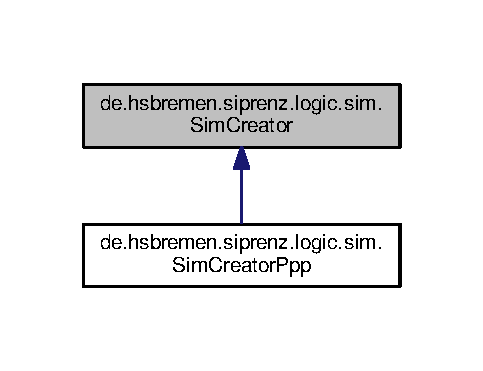
\includegraphics[width=232pt]{interfacede_1_1hsbremen_1_1siprenz_1_1logic_1_1sim_1_1SimCreator__inherit__graph}
\end{center}
\end{figure}
\subsection*{Public Member Functions}
\begin{DoxyCompactItemize}
\item 
\hyperlink{classde_1_1hsbremen_1_1siprenz_1_1model_1_1xml_1_1Simulation}{Simulation} \hyperlink{interfacede_1_1hsbremen_1_1siprenz_1_1logic_1_1sim_1_1SimCreator_af31c0bd004b2b100d9fd2e413cdaeac0}{create} (int nodes\+Count)
\begin{DoxyCompactList}\small\item\em Creates a model for a simulation in ns-\/3. \end{DoxyCompactList}\end{DoxyCompactItemize}


\subsection{Detailed Description}
Interface for creating simulation models. 

\begin{DoxyAuthor}{Author}
David Mittelstädt 
\end{DoxyAuthor}


\subsection{Member Function Documentation}
\index{de\+::hsbremen\+::siprenz\+::logic\+::sim\+::\+Sim\+Creator@{de\+::hsbremen\+::siprenz\+::logic\+::sim\+::\+Sim\+Creator}!create@{create}}
\index{create@{create}!de\+::hsbremen\+::siprenz\+::logic\+::sim\+::\+Sim\+Creator@{de\+::hsbremen\+::siprenz\+::logic\+::sim\+::\+Sim\+Creator}}
\subsubsection[{\texorpdfstring{create(int nodes\+Count)}{create(int nodesCount)}}]{\setlength{\rightskip}{0pt plus 5cm}{\bf Simulation} de.\+hsbremen.\+siprenz.\+logic.\+sim.\+Sim\+Creator.\+create (
\begin{DoxyParamCaption}
\item[{int}]{nodes\+Count}
\end{DoxyParamCaption}
)}\hypertarget{interfacede_1_1hsbremen_1_1siprenz_1_1logic_1_1sim_1_1SimCreator_af31c0bd004b2b100d9fd2e413cdaeac0}{}\label{interfacede_1_1hsbremen_1_1siprenz_1_1logic_1_1sim_1_1SimCreator_af31c0bd004b2b100d9fd2e413cdaeac0}


Creates a model for a simulation in ns-\/3. 


\begin{DoxyParams}{Parameters}
{\em nodes\+Count} & \\
\hline
\end{DoxyParams}
\begin{DoxyReturn}{Returns}
Simulation object 
\end{DoxyReturn}


Implemented in \hyperlink{classde_1_1hsbremen_1_1siprenz_1_1logic_1_1sim_1_1SimCreatorPpp_ad7a34fe3370aca35835f067507883d13}{de.\+hsbremen.\+siprenz.\+logic.\+sim.\+Sim\+Creator\+Ppp}.



The documentation for this interface was generated from the following file\+:\begin{DoxyCompactItemize}
\item 
src/de/hsbremen/siprenz/logic/sim/Sim\+Creator.\+java\end{DoxyCompactItemize}

\hypertarget{classde_1_1hsbremen_1_1siprenz_1_1logic_1_1sim_1_1SimCreatorPpp}{}\section{de.\+hsbremen.\+siprenz.\+logic.\+sim.\+Sim\+Creator\+Ppp Class Reference}
\label{classde_1_1hsbremen_1_1siprenz_1_1logic_1_1sim_1_1SimCreatorPpp}\index{de.\+hsbremen.\+siprenz.\+logic.\+sim.\+Sim\+Creator\+Ppp@{de.\+hsbremen.\+siprenz.\+logic.\+sim.\+Sim\+Creator\+Ppp}}


Implementation of the \hyperlink{interfacede_1_1hsbremen_1_1siprenz_1_1logic_1_1sim_1_1SimCreator}{Sim\+Creator} interface for P2P models in ns-\/3.  




Inheritance diagram for de.\+hsbremen.\+siprenz.\+logic.\+sim.\+Sim\+Creator\+Ppp\+:\nopagebreak
\begin{figure}[H]
\begin{center}
\leavevmode
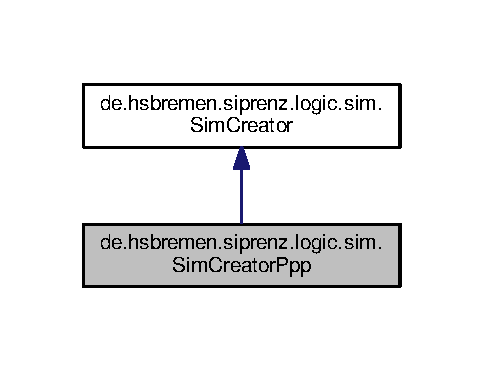
\includegraphics[width=232pt]{classde_1_1hsbremen_1_1siprenz_1_1logic_1_1sim_1_1SimCreatorPpp__inherit__graph}
\end{center}
\end{figure}


Collaboration diagram for de.\+hsbremen.\+siprenz.\+logic.\+sim.\+Sim\+Creator\+Ppp\+:\nopagebreak
\begin{figure}[H]
\begin{center}
\leavevmode
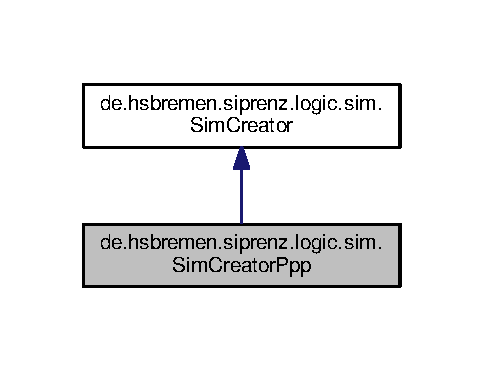
\includegraphics[width=232pt]{classde_1_1hsbremen_1_1siprenz_1_1logic_1_1sim_1_1SimCreatorPpp__coll__graph}
\end{center}
\end{figure}
\subsection*{Public Member Functions}
\begin{DoxyCompactItemize}
\item 
\hyperlink{classde_1_1hsbremen_1_1siprenz_1_1model_1_1xml_1_1Simulation}{Simulation} \hyperlink{classde_1_1hsbremen_1_1siprenz_1_1logic_1_1sim_1_1SimCreatorPpp_ad7a34fe3370aca35835f067507883d13}{create} (int nodes\+Count)
\begin{DoxyCompactList}\small\item\em Creates a model for a simulation in ns-\/3. \end{DoxyCompactList}\end{DoxyCompactItemize}


\subsection{Detailed Description}
Implementation of the \hyperlink{interfacede_1_1hsbremen_1_1siprenz_1_1logic_1_1sim_1_1SimCreator}{Sim\+Creator} interface for P2P models in ns-\/3. 

\begin{DoxyAuthor}{Author}
David Mittelstädt 
\end{DoxyAuthor}


\subsection{Member Function Documentation}
\index{de\+::hsbremen\+::siprenz\+::logic\+::sim\+::\+Sim\+Creator\+Ppp@{de\+::hsbremen\+::siprenz\+::logic\+::sim\+::\+Sim\+Creator\+Ppp}!create@{create}}
\index{create@{create}!de\+::hsbremen\+::siprenz\+::logic\+::sim\+::\+Sim\+Creator\+Ppp@{de\+::hsbremen\+::siprenz\+::logic\+::sim\+::\+Sim\+Creator\+Ppp}}
\subsubsection[{\texorpdfstring{create(int nodes\+Count)}{create(int nodesCount)}}]{\setlength{\rightskip}{0pt plus 5cm}{\bf Simulation} de.\+hsbremen.\+siprenz.\+logic.\+sim.\+Sim\+Creator\+Ppp.\+create (
\begin{DoxyParamCaption}
\item[{int}]{nodes\+Count}
\end{DoxyParamCaption}
)\hspace{0.3cm}{\ttfamily [inline]}}\hypertarget{classde_1_1hsbremen_1_1siprenz_1_1logic_1_1sim_1_1SimCreatorPpp_ad7a34fe3370aca35835f067507883d13}{}\label{classde_1_1hsbremen_1_1siprenz_1_1logic_1_1sim_1_1SimCreatorPpp_ad7a34fe3370aca35835f067507883d13}


Creates a model for a simulation in ns-\/3. 


\begin{DoxyParams}{Parameters}
{\em nodes\+Count} & \\
\hline
\end{DoxyParams}
\begin{DoxyReturn}{Returns}
Simulation object 
\end{DoxyReturn}


Implements \hyperlink{interfacede_1_1hsbremen_1_1siprenz_1_1logic_1_1sim_1_1SimCreator_af31c0bd004b2b100d9fd2e413cdaeac0}{de.\+hsbremen.\+siprenz.\+logic.\+sim.\+Sim\+Creator}.



The documentation for this class was generated from the following file\+:\begin{DoxyCompactItemize}
\item 
src/de/hsbremen/siprenz/logic/sim/Sim\+Creator\+Ppp.\+java\end{DoxyCompactItemize}

\hypertarget{classde_1_1hsbremen_1_1siprenz_1_1logic_1_1sim_1_1SimExecutor}{}\section{de.\+hsbremen.\+siprenz.\+logic.\+sim.\+Sim\+Executor Class Reference}
\label{classde_1_1hsbremen_1_1siprenz_1_1logic_1_1sim_1_1SimExecutor}\index{de.\+hsbremen.\+siprenz.\+logic.\+sim.\+Sim\+Executor@{de.\+hsbremen.\+siprenz.\+logic.\+sim.\+Sim\+Executor}}


Class for executing a simulation.  




Collaboration diagram for de.\+hsbremen.\+siprenz.\+logic.\+sim.\+Sim\+Executor\+:\nopagebreak
\begin{figure}[H]
\begin{center}
\leavevmode
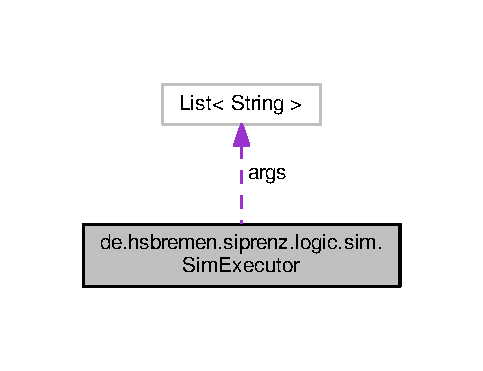
\includegraphics[width=232pt]{classde_1_1hsbremen_1_1siprenz_1_1logic_1_1sim_1_1SimExecutor__coll__graph}
\end{center}
\end{figure}
\subsection*{Public Member Functions}
\begin{DoxyCompactItemize}
\item 
void \hyperlink{classde_1_1hsbremen_1_1siprenz_1_1logic_1_1sim_1_1SimExecutor_ae9a0ff34fd3f911ab69046f847eb5b31}{start} ()\hypertarget{classde_1_1hsbremen_1_1siprenz_1_1logic_1_1sim_1_1SimExecutor_ae9a0ff34fd3f911ab69046f847eb5b31}{}\label{classde_1_1hsbremen_1_1siprenz_1_1logic_1_1sim_1_1SimExecutor_ae9a0ff34fd3f911ab69046f847eb5b31}

\begin{DoxyCompactList}\small\item\em Start a simulation. \end{DoxyCompactList}\end{DoxyCompactItemize}


\subsection{Detailed Description}
Class for executing a simulation. 

Not full implemented

\begin{DoxyAuthor}{Author}
David Mittelstädt 
\end{DoxyAuthor}


The documentation for this class was generated from the following file\+:\begin{DoxyCompactItemize}
\item 
src/de/hsbremen/siprenz/logic/sim/Sim\+Executor.\+java\end{DoxyCompactItemize}

\hypertarget{classde_1_1hsbremen_1_1siprenz_1_1model_1_1xml_1_1Simulation}{}\section{de.\+hsbremen.\+siprenz.\+model.\+xml.\+Simulation Class Reference}
\label{classde_1_1hsbremen_1_1siprenz_1_1model_1_1xml_1_1Simulation}\index{de.\+hsbremen.\+siprenz.\+model.\+xml.\+Simulation@{de.\+hsbremen.\+siprenz.\+model.\+xml.\+Simulation}}


Class for the whole simulation.  


\subsection*{Public Member Functions}
\begin{DoxyCompactItemize}
\item 
\hyperlink{classde_1_1hsbremen_1_1siprenz_1_1model_1_1xml_1_1Global}{Global} \hyperlink{classde_1_1hsbremen_1_1siprenz_1_1model_1_1xml_1_1Simulation_a5de2d2c7931dd9e63c3750308ad7e68a}{get\+Global} ()
\item 
void \hyperlink{classde_1_1hsbremen_1_1siprenz_1_1model_1_1xml_1_1Simulation_a6b9f032eebc383e28bc17c85efb82867}{set\+Global} (\hyperlink{classde_1_1hsbremen_1_1siprenz_1_1model_1_1xml_1_1Global}{Global} global)
\item 
Array\+List$<$ \hyperlink{classde_1_1hsbremen_1_1siprenz_1_1model_1_1xml_1_1Connection}{Connection} $>$ \hyperlink{classde_1_1hsbremen_1_1siprenz_1_1model_1_1xml_1_1Simulation_a3d8f5ba52821c49ec09d7330b28d746c}{get\+Connections} ()
\item 
void \hyperlink{classde_1_1hsbremen_1_1siprenz_1_1model_1_1xml_1_1Simulation_aad199aa4a6175a6c89861437969a8020}{set\+Connections} (Array\+List$<$ \hyperlink{classde_1_1hsbremen_1_1siprenz_1_1model_1_1xml_1_1Connection}{Connection} $>$ connections)
\item 
Array\+List$<$ \hyperlink{classde_1_1hsbremen_1_1siprenz_1_1model_1_1xml_1_1Node}{Node} $>$ \hyperlink{classde_1_1hsbremen_1_1siprenz_1_1model_1_1xml_1_1Simulation_a2a45fc72e1d1c2591dee145090b0f579}{get\+Nodes} ()
\item 
void \hyperlink{classde_1_1hsbremen_1_1siprenz_1_1model_1_1xml_1_1Simulation_add0ed0bfe51af13b276a2aa6e708e7a6}{set\+Nodes} (Array\+List$<$ \hyperlink{classde_1_1hsbremen_1_1siprenz_1_1model_1_1xml_1_1Node}{Node} $>$ nodes)
\end{DoxyCompactItemize}


\subsection{Detailed Description}
Class for the whole simulation. 

\begin{DoxyAuthor}{Author}
David Mittelstädt 
\end{DoxyAuthor}


\subsection{Member Function Documentation}
\index{de\+::hsbremen\+::siprenz\+::model\+::xml\+::\+Simulation@{de\+::hsbremen\+::siprenz\+::model\+::xml\+::\+Simulation}!get\+Connections@{get\+Connections}}
\index{get\+Connections@{get\+Connections}!de\+::hsbremen\+::siprenz\+::model\+::xml\+::\+Simulation@{de\+::hsbremen\+::siprenz\+::model\+::xml\+::\+Simulation}}
\subsubsection[{\texorpdfstring{get\+Connections()}{getConnections()}}]{\setlength{\rightskip}{0pt plus 5cm}Array\+List$<${\bf Connection}$>$ de.\+hsbremen.\+siprenz.\+model.\+xml.\+Simulation.\+get\+Connections (
\begin{DoxyParamCaption}
{}
\end{DoxyParamCaption}
)\hspace{0.3cm}{\ttfamily [inline]}}\hypertarget{classde_1_1hsbremen_1_1siprenz_1_1model_1_1xml_1_1Simulation_a3d8f5ba52821c49ec09d7330b28d746c}{}\label{classde_1_1hsbremen_1_1siprenz_1_1model_1_1xml_1_1Simulation_a3d8f5ba52821c49ec09d7330b28d746c}
\begin{DoxyReturn}{Returns}
All connections of the simulation 
\end{DoxyReturn}
\index{de\+::hsbremen\+::siprenz\+::model\+::xml\+::\+Simulation@{de\+::hsbremen\+::siprenz\+::model\+::xml\+::\+Simulation}!get\+Global@{get\+Global}}
\index{get\+Global@{get\+Global}!de\+::hsbremen\+::siprenz\+::model\+::xml\+::\+Simulation@{de\+::hsbremen\+::siprenz\+::model\+::xml\+::\+Simulation}}
\subsubsection[{\texorpdfstring{get\+Global()}{getGlobal()}}]{\setlength{\rightskip}{0pt plus 5cm}{\bf Global} de.\+hsbremen.\+siprenz.\+model.\+xml.\+Simulation.\+get\+Global (
\begin{DoxyParamCaption}
{}
\end{DoxyParamCaption}
)\hspace{0.3cm}{\ttfamily [inline]}}\hypertarget{classde_1_1hsbremen_1_1siprenz_1_1model_1_1xml_1_1Simulation_a5de2d2c7931dd9e63c3750308ad7e68a}{}\label{classde_1_1hsbremen_1_1siprenz_1_1model_1_1xml_1_1Simulation_a5de2d2c7931dd9e63c3750308ad7e68a}
\begin{DoxyReturn}{Returns}
\hyperlink{classde_1_1hsbremen_1_1siprenz_1_1model_1_1xml_1_1Global}{Global} part of the simulation 
\end{DoxyReturn}
\index{de\+::hsbremen\+::siprenz\+::model\+::xml\+::\+Simulation@{de\+::hsbremen\+::siprenz\+::model\+::xml\+::\+Simulation}!get\+Nodes@{get\+Nodes}}
\index{get\+Nodes@{get\+Nodes}!de\+::hsbremen\+::siprenz\+::model\+::xml\+::\+Simulation@{de\+::hsbremen\+::siprenz\+::model\+::xml\+::\+Simulation}}
\subsubsection[{\texorpdfstring{get\+Nodes()}{getNodes()}}]{\setlength{\rightskip}{0pt plus 5cm}Array\+List$<${\bf Node}$>$ de.\+hsbremen.\+siprenz.\+model.\+xml.\+Simulation.\+get\+Nodes (
\begin{DoxyParamCaption}
{}
\end{DoxyParamCaption}
)\hspace{0.3cm}{\ttfamily [inline]}}\hypertarget{classde_1_1hsbremen_1_1siprenz_1_1model_1_1xml_1_1Simulation_a2a45fc72e1d1c2591dee145090b0f579}{}\label{classde_1_1hsbremen_1_1siprenz_1_1model_1_1xml_1_1Simulation_a2a45fc72e1d1c2591dee145090b0f579}
\begin{DoxyReturn}{Returns}
All nodes of the simulation 
\end{DoxyReturn}
\index{de\+::hsbremen\+::siprenz\+::model\+::xml\+::\+Simulation@{de\+::hsbremen\+::siprenz\+::model\+::xml\+::\+Simulation}!set\+Connections@{set\+Connections}}
\index{set\+Connections@{set\+Connections}!de\+::hsbremen\+::siprenz\+::model\+::xml\+::\+Simulation@{de\+::hsbremen\+::siprenz\+::model\+::xml\+::\+Simulation}}
\subsubsection[{\texorpdfstring{set\+Connections(\+Array\+List$<$ Connection $>$ connections)}{setConnections(ArrayList< Connection > connections)}}]{\setlength{\rightskip}{0pt plus 5cm}void de.\+hsbremen.\+siprenz.\+model.\+xml.\+Simulation.\+set\+Connections (
\begin{DoxyParamCaption}
\item[{Array\+List$<$ {\bf Connection} $>$}]{connections}
\end{DoxyParamCaption}
)\hspace{0.3cm}{\ttfamily [inline]}}\hypertarget{classde_1_1hsbremen_1_1siprenz_1_1model_1_1xml_1_1Simulation_aad199aa4a6175a6c89861437969a8020}{}\label{classde_1_1hsbremen_1_1siprenz_1_1model_1_1xml_1_1Simulation_aad199aa4a6175a6c89861437969a8020}

\begin{DoxyParams}{Parameters}
{\em connections} & All connections of the simulation \\
\hline
\end{DoxyParams}
\index{de\+::hsbremen\+::siprenz\+::model\+::xml\+::\+Simulation@{de\+::hsbremen\+::siprenz\+::model\+::xml\+::\+Simulation}!set\+Global@{set\+Global}}
\index{set\+Global@{set\+Global}!de\+::hsbremen\+::siprenz\+::model\+::xml\+::\+Simulation@{de\+::hsbremen\+::siprenz\+::model\+::xml\+::\+Simulation}}
\subsubsection[{\texorpdfstring{set\+Global(\+Global global)}{setGlobal(Global global)}}]{\setlength{\rightskip}{0pt plus 5cm}void de.\+hsbremen.\+siprenz.\+model.\+xml.\+Simulation.\+set\+Global (
\begin{DoxyParamCaption}
\item[{{\bf Global}}]{global}
\end{DoxyParamCaption}
)\hspace{0.3cm}{\ttfamily [inline]}}\hypertarget{classde_1_1hsbremen_1_1siprenz_1_1model_1_1xml_1_1Simulation_a6b9f032eebc383e28bc17c85efb82867}{}\label{classde_1_1hsbremen_1_1siprenz_1_1model_1_1xml_1_1Simulation_a6b9f032eebc383e28bc17c85efb82867}

\begin{DoxyParams}{Parameters}
{\em global} & \hyperlink{classde_1_1hsbremen_1_1siprenz_1_1model_1_1xml_1_1Global}{Global} part of the simulation \\
\hline
\end{DoxyParams}
\index{de\+::hsbremen\+::siprenz\+::model\+::xml\+::\+Simulation@{de\+::hsbremen\+::siprenz\+::model\+::xml\+::\+Simulation}!set\+Nodes@{set\+Nodes}}
\index{set\+Nodes@{set\+Nodes}!de\+::hsbremen\+::siprenz\+::model\+::xml\+::\+Simulation@{de\+::hsbremen\+::siprenz\+::model\+::xml\+::\+Simulation}}
\subsubsection[{\texorpdfstring{set\+Nodes(\+Array\+List$<$ Node $>$ nodes)}{setNodes(ArrayList< Node > nodes)}}]{\setlength{\rightskip}{0pt plus 5cm}void de.\+hsbremen.\+siprenz.\+model.\+xml.\+Simulation.\+set\+Nodes (
\begin{DoxyParamCaption}
\item[{Array\+List$<$ {\bf Node} $>$}]{nodes}
\end{DoxyParamCaption}
)\hspace{0.3cm}{\ttfamily [inline]}}\hypertarget{classde_1_1hsbremen_1_1siprenz_1_1model_1_1xml_1_1Simulation_add0ed0bfe51af13b276a2aa6e708e7a6}{}\label{classde_1_1hsbremen_1_1siprenz_1_1model_1_1xml_1_1Simulation_add0ed0bfe51af13b276a2aa6e708e7a6}

\begin{DoxyParams}{Parameters}
{\em nodes} & All nodes of the simulation \\
\hline
\end{DoxyParams}


The documentation for this class was generated from the following file\+:\begin{DoxyCompactItemize}
\item 
src/de/hsbremen/siprenz/model/xml/Simulation.\+java\end{DoxyCompactItemize}

\hypertarget{classde_1_1hsbremen_1_1siprenz_1_1utils_1_1StreamUtils}{}\section{de.\+hsbremen.\+siprenz.\+utils.\+Stream\+Utils Class Reference}
\label{classde_1_1hsbremen_1_1siprenz_1_1utils_1_1StreamUtils}\index{de.\+hsbremen.\+siprenz.\+utils.\+Stream\+Utils@{de.\+hsbremen.\+siprenz.\+utils.\+Stream\+Utils}}


Class for some stream operations.  


\subsection*{Static Public Member Functions}
\begin{DoxyCompactItemize}
\item 
static String \hyperlink{classde_1_1hsbremen_1_1siprenz_1_1utils_1_1StreamUtils_ab71abe87e68127839ad2800ba0912c82}{get\+String\+From\+Input\+Stream} (Input\+Stream input\+Stream)
\begin{DoxyCompactList}\small\item\em Creates a String from input\+Strem. \end{DoxyCompactList}\end{DoxyCompactItemize}


\subsection{Detailed Description}
Class for some stream operations. 

\begin{DoxyAuthor}{Author}
David Mittelstädt 
\end{DoxyAuthor}


\subsection{Member Function Documentation}
\index{de\+::hsbremen\+::siprenz\+::utils\+::\+Stream\+Utils@{de\+::hsbremen\+::siprenz\+::utils\+::\+Stream\+Utils}!get\+String\+From\+Input\+Stream@{get\+String\+From\+Input\+Stream}}
\index{get\+String\+From\+Input\+Stream@{get\+String\+From\+Input\+Stream}!de\+::hsbremen\+::siprenz\+::utils\+::\+Stream\+Utils@{de\+::hsbremen\+::siprenz\+::utils\+::\+Stream\+Utils}}
\subsubsection[{\texorpdfstring{get\+String\+From\+Input\+Stream(\+Input\+Stream input\+Stream)}{getStringFromInputStream(InputStream inputStream)}}]{\setlength{\rightskip}{0pt plus 5cm}static String de.\+hsbremen.\+siprenz.\+utils.\+Stream\+Utils.\+get\+String\+From\+Input\+Stream (
\begin{DoxyParamCaption}
\item[{Input\+Stream}]{input\+Stream}
\end{DoxyParamCaption}
)\hspace{0.3cm}{\ttfamily [inline]}, {\ttfamily [static]}}\hypertarget{classde_1_1hsbremen_1_1siprenz_1_1utils_1_1StreamUtils_ab71abe87e68127839ad2800ba0912c82}{}\label{classde_1_1hsbremen_1_1siprenz_1_1utils_1_1StreamUtils_ab71abe87e68127839ad2800ba0912c82}


Creates a String from input\+Strem. 


\begin{DoxyParams}{Parameters}
{\em input\+Stream} & Input\+Stream \\
\hline
\end{DoxyParams}
\begin{DoxyReturn}{Returns}
String 
\end{DoxyReturn}


The documentation for this class was generated from the following file\+:\begin{DoxyCompactItemize}
\item 
src/de/hsbremen/siprenz/utils/Stream\+Utils.\+java\end{DoxyCompactItemize}

\hypertarget{classStringHelper}{}\section{String\+Helper Class Reference}
\label{classStringHelper}\index{String\+Helper@{String\+Helper}}
\subsection*{Static Public Member Functions}
\begin{DoxyCompactItemize}
\item 
static std\+::string {\bfseries to\+String} (double const \&value)\hypertarget{classStringHelper_a9b19e4812a60dcc1c3f2706db473bad7}{}\label{classStringHelper_a9b19e4812a60dcc1c3f2706db473bad7}

\end{DoxyCompactItemize}


The documentation for this class was generated from the following files\+:\begin{DoxyCompactItemize}
\item 
src/res/string-\/helper.\+h\item 
src/res/string-\/helper.\+cc\end{DoxyCompactItemize}

\hypertarget{classde_1_1hsbremen_1_1siprenz_1_1logic_1_1xml_1_1XmlParser}{}\section{de.\+hsbremen.\+siprenz.\+logic.\+xml.\+Xml\+Parser Class Reference}
\label{classde_1_1hsbremen_1_1siprenz_1_1logic_1_1xml_1_1XmlParser}\index{de.\+hsbremen.\+siprenz.\+logic.\+xml.\+Xml\+Parser@{de.\+hsbremen.\+siprenz.\+logic.\+xml.\+Xml\+Parser}}


Class for parsing the X\+ML.  


\subsection*{Public Member Functions}
\begin{DoxyCompactItemize}
\item 
void \hyperlink{classde_1_1hsbremen_1_1siprenz_1_1logic_1_1xml_1_1XmlParser_ac45ff895eebf7ad76196917c92eb03c8}{write} (\hyperlink{classde_1_1hsbremen_1_1siprenz_1_1model_1_1xml_1_1Simulation}{Simulation} simulation, String path\+Name)
\begin{DoxyCompactList}\small\item\em Writes simulation to X\+ML. \end{DoxyCompactList}\item 
\hyperlink{classde_1_1hsbremen_1_1siprenz_1_1model_1_1xml_1_1Simulation}{Simulation} \hyperlink{classde_1_1hsbremen_1_1siprenz_1_1logic_1_1xml_1_1XmlParser_a1847162a8559bae6b4cccc30fd86c989}{read} (String path\+Name)
\begin{DoxyCompactList}\small\item\em Reads simulation from X\+ML. \end{DoxyCompactList}\end{DoxyCompactItemize}


\subsection{Detailed Description}
Class for parsing the X\+ML. 

This class is used for parsing the model from a X\+ML file and writing a model to a X\+ML file.

\begin{DoxyAuthor}{Author}
David Mittelstädt 
\end{DoxyAuthor}


\subsection{Member Function Documentation}
\index{de\+::hsbremen\+::siprenz\+::logic\+::xml\+::\+Xml\+Parser@{de\+::hsbremen\+::siprenz\+::logic\+::xml\+::\+Xml\+Parser}!read@{read}}
\index{read@{read}!de\+::hsbremen\+::siprenz\+::logic\+::xml\+::\+Xml\+Parser@{de\+::hsbremen\+::siprenz\+::logic\+::xml\+::\+Xml\+Parser}}
\subsubsection[{\texorpdfstring{read(\+String path\+Name)}{read(String pathName)}}]{\setlength{\rightskip}{0pt plus 5cm}{\bf Simulation} de.\+hsbremen.\+siprenz.\+logic.\+xml.\+Xml\+Parser.\+read (
\begin{DoxyParamCaption}
\item[{String}]{path\+Name}
\end{DoxyParamCaption}
)\hspace{0.3cm}{\ttfamily [inline]}}\hypertarget{classde_1_1hsbremen_1_1siprenz_1_1logic_1_1xml_1_1XmlParser_a1847162a8559bae6b4cccc30fd86c989}{}\label{classde_1_1hsbremen_1_1siprenz_1_1logic_1_1xml_1_1XmlParser_a1847162a8559bae6b4cccc30fd86c989}


Reads simulation from X\+ML. 

This functions reads a simulation model from X\+ML file.


\begin{DoxyParams}{Parameters}
{\em path\+Name} & full path of the X\+ML file to read \\
\hline
\end{DoxyParams}
\begin{DoxyReturn}{Returns}
simulation 
\end{DoxyReturn}
\index{de\+::hsbremen\+::siprenz\+::logic\+::xml\+::\+Xml\+Parser@{de\+::hsbremen\+::siprenz\+::logic\+::xml\+::\+Xml\+Parser}!write@{write}}
\index{write@{write}!de\+::hsbremen\+::siprenz\+::logic\+::xml\+::\+Xml\+Parser@{de\+::hsbremen\+::siprenz\+::logic\+::xml\+::\+Xml\+Parser}}
\subsubsection[{\texorpdfstring{write(\+Simulation simulation, String path\+Name)}{write(Simulation simulation, String pathName)}}]{\setlength{\rightskip}{0pt plus 5cm}void de.\+hsbremen.\+siprenz.\+logic.\+xml.\+Xml\+Parser.\+write (
\begin{DoxyParamCaption}
\item[{{\bf Simulation}}]{simulation, }
\item[{String}]{path\+Name}
\end{DoxyParamCaption}
)\hspace{0.3cm}{\ttfamily [inline]}}\hypertarget{classde_1_1hsbremen_1_1siprenz_1_1logic_1_1xml_1_1XmlParser_ac45ff895eebf7ad76196917c92eb03c8}{}\label{classde_1_1hsbremen_1_1siprenz_1_1logic_1_1xml_1_1XmlParser_ac45ff895eebf7ad76196917c92eb03c8}


Writes simulation to X\+ML. 

This function writes a simulation model to a X\+Ml File.


\begin{DoxyParams}{Parameters}
{\em simulation} & Simulation to write to X\+ML \\
\hline
{\em path\+Name} & Name of the full path to save the X\+ML \\
\hline
\end{DoxyParams}


The documentation for this class was generated from the following file\+:\begin{DoxyCompactItemize}
\item 
src/de/hsbremen/siprenz/logic/xml/Xml\+Parser.\+java\end{DoxyCompactItemize}

\hypertarget{classde_1_1hsbremen_1_1siprenz_1_1model_1_1gen_1_1XmlProps}{}\section{de.\+hsbremen.\+siprenz.\+model.\+gen.\+Xml\+Props Class Reference}
\label{classde_1_1hsbremen_1_1siprenz_1_1model_1_1gen_1_1XmlProps}\index{de.\+hsbremen.\+siprenz.\+model.\+gen.\+Xml\+Props@{de.\+hsbremen.\+siprenz.\+model.\+gen.\+Xml\+Props}}


Class representing X\+ML properties.  


\subsection*{Public Member Functions}
\begin{DoxyCompactItemize}
\item 
\hyperlink{classde_1_1hsbremen_1_1siprenz_1_1model_1_1gen_1_1XmlProps_a27d294cb758c5cc9e345b34fc3767b82}{Xml\+Props} (int nodes\+Count, String output\+File)
\begin{DoxyCompactList}\small\item\em Constructor. \end{DoxyCompactList}\item 
int \hyperlink{classde_1_1hsbremen_1_1siprenz_1_1model_1_1gen_1_1XmlProps_ac4d29f604c4fb52a75c07e74f692dac7}{get\+Nodes\+Count} ()
\item 
void \hyperlink{classde_1_1hsbremen_1_1siprenz_1_1model_1_1gen_1_1XmlProps_a2a4b152e6c5dcf3152cf1dd1f93d55c6}{set\+Nodes\+Count} (int nodes\+Count)
\item 
String \hyperlink{classde_1_1hsbremen_1_1siprenz_1_1model_1_1gen_1_1XmlProps_a231e270615fd3fa569d810bb3a24670f}{get\+Output\+File} ()
\item 
void \hyperlink{classde_1_1hsbremen_1_1siprenz_1_1model_1_1gen_1_1XmlProps_a8f29f92cfad597322f352b2647d64053}{set\+Output\+File} (String out\+File)
\end{DoxyCompactItemize}


\subsection{Detailed Description}
Class representing X\+ML properties. 

\begin{DoxyAuthor}{Author}
David Mittelstädt 
\end{DoxyAuthor}


\subsection{Constructor \& Destructor Documentation}
\index{de\+::hsbremen\+::siprenz\+::model\+::gen\+::\+Xml\+Props@{de\+::hsbremen\+::siprenz\+::model\+::gen\+::\+Xml\+Props}!Xml\+Props@{Xml\+Props}}
\index{Xml\+Props@{Xml\+Props}!de\+::hsbremen\+::siprenz\+::model\+::gen\+::\+Xml\+Props@{de\+::hsbremen\+::siprenz\+::model\+::gen\+::\+Xml\+Props}}
\subsubsection[{\texorpdfstring{Xml\+Props(int nodes\+Count, String output\+File)}{XmlProps(int nodesCount, String outputFile)}}]{\setlength{\rightskip}{0pt plus 5cm}de.\+hsbremen.\+siprenz.\+model.\+gen.\+Xml\+Props.\+Xml\+Props (
\begin{DoxyParamCaption}
\item[{int}]{nodes\+Count, }
\item[{String}]{output\+File}
\end{DoxyParamCaption}
)\hspace{0.3cm}{\ttfamily [inline]}}\hypertarget{classde_1_1hsbremen_1_1siprenz_1_1model_1_1gen_1_1XmlProps_a27d294cb758c5cc9e345b34fc3767b82}{}\label{classde_1_1hsbremen_1_1siprenz_1_1model_1_1gen_1_1XmlProps_a27d294cb758c5cc9e345b34fc3767b82}


Constructor. 


\begin{DoxyParams}{Parameters}
{\em nodes\+Count} & Number of nodes \\
\hline
{\em output\+File} & Name of the output file \\
\hline
\end{DoxyParams}


\subsection{Member Function Documentation}
\index{de\+::hsbremen\+::siprenz\+::model\+::gen\+::\+Xml\+Props@{de\+::hsbremen\+::siprenz\+::model\+::gen\+::\+Xml\+Props}!get\+Nodes\+Count@{get\+Nodes\+Count}}
\index{get\+Nodes\+Count@{get\+Nodes\+Count}!de\+::hsbremen\+::siprenz\+::model\+::gen\+::\+Xml\+Props@{de\+::hsbremen\+::siprenz\+::model\+::gen\+::\+Xml\+Props}}
\subsubsection[{\texorpdfstring{get\+Nodes\+Count()}{getNodesCount()}}]{\setlength{\rightskip}{0pt plus 5cm}int de.\+hsbremen.\+siprenz.\+model.\+gen.\+Xml\+Props.\+get\+Nodes\+Count (
\begin{DoxyParamCaption}
{}
\end{DoxyParamCaption}
)\hspace{0.3cm}{\ttfamily [inline]}}\hypertarget{classde_1_1hsbremen_1_1siprenz_1_1model_1_1gen_1_1XmlProps_ac4d29f604c4fb52a75c07e74f692dac7}{}\label{classde_1_1hsbremen_1_1siprenz_1_1model_1_1gen_1_1XmlProps_ac4d29f604c4fb52a75c07e74f692dac7}
\begin{DoxyReturn}{Returns}
Number of nodes 
\end{DoxyReturn}
\index{de\+::hsbremen\+::siprenz\+::model\+::gen\+::\+Xml\+Props@{de\+::hsbremen\+::siprenz\+::model\+::gen\+::\+Xml\+Props}!get\+Output\+File@{get\+Output\+File}}
\index{get\+Output\+File@{get\+Output\+File}!de\+::hsbremen\+::siprenz\+::model\+::gen\+::\+Xml\+Props@{de\+::hsbremen\+::siprenz\+::model\+::gen\+::\+Xml\+Props}}
\subsubsection[{\texorpdfstring{get\+Output\+File()}{getOutputFile()}}]{\setlength{\rightskip}{0pt plus 5cm}String de.\+hsbremen.\+siprenz.\+model.\+gen.\+Xml\+Props.\+get\+Output\+File (
\begin{DoxyParamCaption}
{}
\end{DoxyParamCaption}
)\hspace{0.3cm}{\ttfamily [inline]}}\hypertarget{classde_1_1hsbremen_1_1siprenz_1_1model_1_1gen_1_1XmlProps_a231e270615fd3fa569d810bb3a24670f}{}\label{classde_1_1hsbremen_1_1siprenz_1_1model_1_1gen_1_1XmlProps_a231e270615fd3fa569d810bb3a24670f}
\begin{DoxyReturn}{Returns}
Name of the output file 
\end{DoxyReturn}
\index{de\+::hsbremen\+::siprenz\+::model\+::gen\+::\+Xml\+Props@{de\+::hsbremen\+::siprenz\+::model\+::gen\+::\+Xml\+Props}!set\+Nodes\+Count@{set\+Nodes\+Count}}
\index{set\+Nodes\+Count@{set\+Nodes\+Count}!de\+::hsbremen\+::siprenz\+::model\+::gen\+::\+Xml\+Props@{de\+::hsbremen\+::siprenz\+::model\+::gen\+::\+Xml\+Props}}
\subsubsection[{\texorpdfstring{set\+Nodes\+Count(int nodes\+Count)}{setNodesCount(int nodesCount)}}]{\setlength{\rightskip}{0pt plus 5cm}void de.\+hsbremen.\+siprenz.\+model.\+gen.\+Xml\+Props.\+set\+Nodes\+Count (
\begin{DoxyParamCaption}
\item[{int}]{nodes\+Count}
\end{DoxyParamCaption}
)\hspace{0.3cm}{\ttfamily [inline]}}\hypertarget{classde_1_1hsbremen_1_1siprenz_1_1model_1_1gen_1_1XmlProps_a2a4b152e6c5dcf3152cf1dd1f93d55c6}{}\label{classde_1_1hsbremen_1_1siprenz_1_1model_1_1gen_1_1XmlProps_a2a4b152e6c5dcf3152cf1dd1f93d55c6}

\begin{DoxyParams}{Parameters}
{\em nodes\+Count} & Number of nodes \\
\hline
\end{DoxyParams}
\index{de\+::hsbremen\+::siprenz\+::model\+::gen\+::\+Xml\+Props@{de\+::hsbremen\+::siprenz\+::model\+::gen\+::\+Xml\+Props}!set\+Output\+File@{set\+Output\+File}}
\index{set\+Output\+File@{set\+Output\+File}!de\+::hsbremen\+::siprenz\+::model\+::gen\+::\+Xml\+Props@{de\+::hsbremen\+::siprenz\+::model\+::gen\+::\+Xml\+Props}}
\subsubsection[{\texorpdfstring{set\+Output\+File(\+String out\+File)}{setOutputFile(String outFile)}}]{\setlength{\rightskip}{0pt plus 5cm}void de.\+hsbremen.\+siprenz.\+model.\+gen.\+Xml\+Props.\+set\+Output\+File (
\begin{DoxyParamCaption}
\item[{String}]{out\+File}
\end{DoxyParamCaption}
)\hspace{0.3cm}{\ttfamily [inline]}}\hypertarget{classde_1_1hsbremen_1_1siprenz_1_1model_1_1gen_1_1XmlProps_a8f29f92cfad597322f352b2647d64053}{}\label{classde_1_1hsbremen_1_1siprenz_1_1model_1_1gen_1_1XmlProps_a8f29f92cfad597322f352b2647d64053}

\begin{DoxyParams}{Parameters}
{\em out\+File} & Name of the output file \\
\hline
\end{DoxyParams}


The documentation for this class was generated from the following file\+:\begin{DoxyCompactItemize}
\item 
src/de/hsbremen/siprenz/model/gen/Xml\+Props.\+java\end{DoxyCompactItemize}

%--- End generated contents ---

% Index
\backmatter
\newpage
\phantomsection
\clearemptydoublepage
\addcontentsline{toc}{chapter}{Index}
\printindex

\end{document}
